%==============================================================================
% @author Clinton Freeman <freeman@cs.unc.edu>
% @date 09/19/2013
%==============================================================================

\documentclass{article}

\usepackage{fullpage}
\usepackage{amsfonts}
\usepackage{amssymb}
\usepackage{amsmath}
\usepackage{amsthm}
\usepackage[usenames,dvipsnames,svgnames,table]{xcolor}
\usepackage[labelfont=bf]{caption}
\usepackage{url}
\usepackage[linktocpage=true]{hyperref}
\usepackage{algorithm}
\usepackage[noend]{algpseudocode}
\usepackage{esvect}
\usepackage{longtable}
\usepackage{enumitem}
\usepackage{mdframed}
\usepackage{titlesec}
\usepackage{etoolbox}
\usepackage{float}
\usepackage{fancybox}
\usepackage{graphicx}
\usepackage{tabularx}
\usepackage{wrapfig}
\usepackage{booktabs}
\usepackage{tikz}
\usepackage{calc}
\usepackage{placeins}
\usepackage{xcolor}
\usepackage{rotating}
\usepackage[nocompress]{cite}

\definecolor{algback}{rgb}{0.95, 0.95, 0.95}

\usetikzlibrary{shadows, calc, decorations.pathmorphing, shapes, arrows.new}

\hypersetup {
    colorlinks = true,
    linkcolor = {blue},
    citecolor = {blue},
    urlcolor = {blue}
}

\definecolor{keyword}{HTML}{445588}

\newtheorem{theorem}{Theorem}
\newtheorem{corollary}{Corollary}
\newtheorem{lemma}{Lemma}
\newtheorem{invariant}{Invariant}
\theoremstyle{definition}
\newtheorem{definition}{Definition}

\renewcommand{\algorithmicrequire}{\textbf{Input:}}
\renewcommand{\algorithmicensure}{\textbf{Output:}}

\newcommand{\floor}[1]{\left\lfloor #1 \right\rfloor}
\newcommand{\ceiling}[1]{\left\lceil #1 \right\rceil}


\newcommand{\tightoverset}[2]{
    \mathop{#2}\limits^{\vbox to -.8ex{\kern-0.7ex\hbox{$#1$}\vss}}
}

\newcommand{\tikzoverset}[2]{%
  \tikz[baseline=(X.base),inner sep=0pt,outer sep=0pt]{%
    \node[inner sep=0pt,outer sep=0pt] (X) {$#2$};
    \node[yshift=1pt] at (X.north) {$#1$};
}}

\newlength{\mOLineLength}
\newcommand{\mOLine}[1]{
    \overset{
        \setlength{\mOLineLength}{\widthof{#1}}
        \begin{tikzpicture}
            \draw [-to new, arrow head = 1.6pt, line width=0.5pt] (0, 0) --
            +(0.8\mOLineLength, 0);
        \end{tikzpicture}
    }{#1}
}

\newlength{\mRayLength}
\newcommand{\mRay}[1]{
    \tightoverset{
    \setlength{\mRayLength}{\widthof{#1}}
    \begin{tikzpicture}
        \draw [* new-to new, arrow head = 1.6pt, line width=0.5pt]
        (0, 0) -- +(0.8\mRayLength, 0);
        %\filldraw (0,0) circle (0.6pt);
        %\draw [-angle 45 new, arrow head = 2.75pt, line width=0.4pt] (0, 0) --
        %+(0.8\mOLineLength, 0);
    \end{tikzpicture}
    }{\mathrm{#1}}
}

\newlength{\mSegLength}
\newcommand{\mSeg}[1]{
    \tightoverset{
    \setlength{\mSegLength}{\widthof{#1}}
    \begin{tikzpicture}
        \draw [* new-* new, arrow head = 1.6pt] (0, 0) -- +(0.8\mSegLength,
        0);
    \end{tikzpicture}
    }{\mathrm{#1}}
}

\newcommand{\mR}[1]{\mathbb{R}^{#1}}
\newcommand{\mZ}[1]{\mathbb{Z}^{#1}}
\newcommand{\mPoint}[1]{\mathrm{#1}}
\newcommand{\mPt}[1]{\mPoint{#1}}
\newcommand{\mVector}[1]{\mathbf{#1}}
\newcommand{\mVc}[1]{\mVector{#1}}
\newcommand{\mULine}[1]{\tightoverset{\leftrightarrow}{\mathrm{#1}}}
\newcommand{\mMatrix}[1]{\mathbf{#1}}
\newcommand{\mMt}[1]{\mMatrix{#1}}
\newcommand{\mPlane}[1]{\mathrm{#1}}
\newcommand{\mPolygon}[1]{\mathrm{#1}}
\newcommand{\mPolytope}[1]{\mathrm{#1}}
\newcommand{\mSet}[1]{\mathrm{#1}}
\newcommand{\mField}[1]{\mathrm{#1}}
\newcommand{\mCompound}[1]{\mathrm{#1}}
\newcommand{\mIntHull}[1]{\text{IH}(#1)}
\newcommand{\mBoundary}[1]{\partial #1}
\newcommand{\mTernary}[3]{\left( #1 \right) \text{?} #2 \text{:} #3}

\long\def\ignore#1{\relax}

\def\tomath#1{\relax\ifmmode#1\else$#1$\fi}

\def\th{{\rm th}}
\def\inv{^{-1}}
\def\degrees{\tomath{{}^\circ}}
\let\degree=\degrees
\def\lf{\left}\def\rt{\right}

\def\rangeone#1#2{\rangethree{#1}12{#2}}
\def\rangetwo#1#2#3{\tomath{{#1}_{#2},\ldots,{#1}_{#3}}}
\def\rangethree#1#2#3#4{\tomath{{#1}_{#2},{#1}_{#3},\ldots,{#1}_{#4}}}
\let\range=\rangetwo
\def\setone#1#2{\setthree{#1}12{#2}}
\def\settwo#1#2#3{\tomath{\{{#1}_{#2},\ldots,{#1}_{#3}\}}}
\def\setthree#1#2#3#4{\tomath{\{{#1}_{#2},{#1}_{#3},\ldots,{#1}_{#4}\}}}

\def\oldO{
\def\Om(##1){{\tomath{\Omega(##1)}}}
\def\Th(##1){{\tomath{\Theta(##1)}}}
\def\Ologn{\O(\log n)}
\def\Onlogn{\O(n\log n)}
\def\O(##1){{\tomath{O(##1)}}}
\def\On##1{\O(n^{##1})}
}

\def\Om#1{{\tomath{\Omega(#1)}}}
\def\Th#1{{\tomath{\Theta(#1)}}}
\def\Ologn{\O{\log n}}
\def\Onlogn{\O{n\log n}}
\def\O#1{{\tomath{O(#1)}}}
\def\On#1{\O{n^{#1}}}


\def\Case#1{\noindent {\bf Case #1:\/ }}
\def\NP{{\sl NP}}
\def\R{\tomath{{\cal R}}}

\def\etal{{et al.{}}}
\def\fourldots{\mathinner{\ldotp\ldotp\ldotp\ldotp}}
\def\fourdots{\relax\ifmmode
    \fourldots\else$\mathsurround=0pt \fourldots\,$\fi
    \spacefactor=3000}


\def\nopar#1\par{}
\def\slw #1 {{\sl #1 }}
\def\itw #1 {{\it #1 }}
\def\ttw #1 {{\tt #1 }}
\def\scw #1 {{\sc #1 }}
\def\bfw #1 {{\bf #1 }}
\let\bw=\bfw
\def\calw #1 {\tomath{{\cal #1}} }
\def\calv#1{\tomath{{\cal #1}}}

\def\slug{\vrule height 4pt depth 0pt width 4pt}

\def\joinrel{\mathrel{\mkern-4mu}}% fix longrightarrow et c.
\def\ray#1{\hbox{\vbox{\offinterlineskip\setbox0\hbox{$#1$}
    \hbox to \wd0{\hss$\rightharpoonup$\hss}\vskip-1.0pt\box0}}}
\def\lin#1{\hbox{\vbox{\offinterlineskip\setbox0\hbox{$#1$}
    \hbox to \wd0{\hss$\leftrightarrow$\hss}\vskip-1.0pt\box0}}}
\def\seg#1{\tomath{\overline{#1}}}

\def\paper{paper}% for changing papers to thesis chapters

\long\def\comm#1{\ignorespaces}
\def\comments{\long\def\comm##1{\message{COMMENT: ##1}{\bf(( ##1 ))}}}

%\hyphenation{half-space}

\def\raggedcenter{\advance\leftskip by 0pt plus 40em\rightskip=\leftskip
   \parfillskip=0pt \spaceskip=.3333em \xspaceskip=.5em
   \pretolerance=9999 \tolerance=9999
   \hyphenpenalty=9999 \exhyphenpenalty=9999 }

\long\def\tthdump#1{#1} % Do nothing. The following are not done for TtH.
\tthdump{%
%\input Gmacro2.tex
}
 
\newcommand\quelle[1]{{%
      \unskip\nobreak\hfil\penalty50
      \hskip2em\hbox{}\nobreak\hfil#1%
      \parfillskip=0pt \finalhyphendemerits=0 \par}}


\newcounter{proofc}
\renewcommand\theproofc{\arabic{proofc}. }
\DeclareRobustCommand\stepproofc{\refstepcounter{proofc}\theproofc}
\newenvironment{twoproof}{\noindent \emph{Proof.} \\[0.5em]
\tabular{@{\stepproofc}p{2.5in}p{3.25in}}}{\endtabular \\
\quelle{$\square$}\setcounter{proofc}{0}}

\newcounter{sarrow}
\newcommand\xrsquigarrow[1]{%
\stepcounter{sarrow}%
\mathrel{\begin{tikzpicture}[baseline= {( $ (current bounding box.south) + (0,-0.5ex) $ )}]
\node[inner sep=.5ex] (\thesarrow) {$\scriptstyle #1$};
\path[draw,<-,decorate,
  decoration={zigzag,amplitude=0.7pt,segment length=1.2mm,pre=lineto,pre length=4pt}]
    (\thesarrow.south east) -- (\thesarrow.south west);
\end{tikzpicture}}%
}


% code adapted from http://tex.stackexchange.com/a/11483/3954

% some parameters for customization
\def\shadowshift{0pt,0pt}
\def\shadowradius{6pt}

\colorlet{innercolor}{black!60}
\colorlet{outercolor}{gray!05}

% this draws a shadow under a rectangle node
\newcommand\drawshadow[1]{
    \begin{pgfonlayer}{shadow}
        \shade[outercolor,inner color=innercolor,outer color=outercolor] ($(#1.south west)+(\shadowshift)+(\shadowradius/2,\shadowradius/2)$) circle (\shadowradius);
        \shade[outercolor,inner color=innercolor,outer color=outercolor] ($(#1.north west)+(\shadowshift)+(\shadowradius/2,-\shadowradius/2)$) circle (\shadowradius);
        \shade[outercolor,inner color=innercolor,outer color=outercolor] ($(#1.south east)+(\shadowshift)+(-\shadowradius/2,\shadowradius/2)$) circle (\shadowradius);
        \shade[outercolor,inner color=innercolor,outer color=outercolor] ($(#1.north east)+(\shadowshift)+(-\shadowradius/2,-\shadowradius/2)$) circle (\shadowradius);
        \shade[top color=innercolor,bottom color=outercolor] ($(#1.south west)+(\shadowshift)+(\shadowradius/2,-\shadowradius/2)$) rectangle ($(#1.south east)+(\shadowshift)+(-\shadowradius/2,\shadowradius/2)$);
        \shade[left color=innercolor,right color=outercolor] ($(#1.south east)+(\shadowshift)+(-\shadowradius/2,\shadowradius/2)$) rectangle ($(#1.north east)+(\shadowshift)+(\shadowradius/2,-\shadowradius/2)$);
        \shade[bottom color=innercolor,top color=outercolor] ($(#1.north west)+(\shadowshift)+(\shadowradius/2,-\shadowradius/2)$) rectangle ($(#1.north east)+(\shadowshift)+(-\shadowradius/2,\shadowradius/2)$);
        \shade[outercolor,right color=innercolor,left color=outercolor] ($(#1.south west)+(\shadowshift)+(-\shadowradius/2,\shadowradius/2)$) rectangle ($(#1.north west)+(\shadowshift)+(\shadowradius/2,-\shadowradius/2)$);
        \filldraw ($(#1.south west)+(\shadowshift)+(\shadowradius/2,\shadowradius/2)$) rectangle ($(#1.north east)+(\shadowshift)-(\shadowradius/2,\shadowradius/2)$);
    \end{pgfonlayer}
}

% create a shadow layer, so that we don't need to worry about overdrawing other things
\pgfdeclarelayer{shadow} 
\pgfsetlayers{shadow,main}


\newcommand\shadowimage[2][]{%
\begin{tikzpicture}
\node[anchor=south west,inner sep=0] (image) at (0,0) {\includegraphics[#1]{#2}};
\drawshadow{image}
\end{tikzpicture}}

\definecolor{answerColor}{RGB}{245, 245, 245}
\definecolor{titleColor}{RGB}{225, 225, 225}
\mdfdefinestyle{answer} {
    backgroundcolor = answerColor,
    linecolor = answerColor,
    skipabove = 8pt,
    skipbelow = 8pt,
    splittopskip = 22pt,
    splitbottomskip = \baselineskip,
    innertopmargin = 0.75em,
    innerbottommargin = 0.75em,
    innerrightmargin = 0.75em,
    innerleftmargin = 0.75em,
    frametitlealignment=\center,
    frametitlebackgroundcolor=titleColor
}

\definecolor{cBack}{rgb}{0.95, 0.95, 0.95}
\usepackage{listings}
\lstset {
        basicstyle = \footnotesize\ttfamily,
        backgroundcolor = \color{cBack},
        %numbers = left,
        numberstyle = \tiny,
        %stepnumber = 2,
        numbersep = 5pt,
        tabsize = 2,
        extendedchars = true,
        breaklines = true,
        keywordstyle = \color{red},
        frame = b,
        stringstyle = \color{white}\ttfamily,
        showspaces = false,
        showtabs = false,
        frame = shadowbox,
        framexleftmargin = 8pt,
        framexrightmargin = 8pt, 
        framexbottommargin = 8pt,
        framextopmargin = 8pt,  
        aboveskip = 12pt,
        belowskip = 12pt,
        showstringspaces = false
}

\lstloadlanguages {
        C++
}

\DeclareCaptionFont{white}{\color{white}}
\DeclareCaptionFormat{listing}{\colorbox[rgb]{0.4, 0.4,
0.4}{\parbox{\textwidth}{\hspace{8pt}#1#2#3}}}
\captionsetup[lstlisting]{format=listing,labelfont=white,textfont=white, singlelinecheck=false, margin=0pt, font={sf,bf,footnotesize}}

\def\tomath#1{\relax\ifmmode#1\else$#1$\fi}
\def\opName#1{\hbox{\tt{\textsc{#1}}}}
\def\op#1(#2){\tomath{\opName{#1}(#2)}}

\def\deg(#1){\tomath{\mathord{ \large \textcircled{\small \tomath{#1}} \normalsize }}}

%\linespread{1.5}

\title{A Geometric Workbench for Degree-Driven Algorithm Design}
\author{
        Clinton Freeman \\
        \texttt{freeman@cs.unc.edu}
        \and
        Jack Snoeyink \\
    \texttt{snoeyink@cs.unc.edu}
}

\begin{document}

\maketitle

%==============================================================================

\begin{abstract}
Millman built a C++ library (DDAD) to facilitate implementing algorithms with
low-degree predicates. Our workbench extends DDAD with a visual event system and
provides a standalone GUI that can generate input data and render algorithm
execution. The visual event system is built on the concept of observable
geometry which we combine with a traditional MVC architecture to create a
powerful API for visualizing geometric algorithms. We demonstrate the
workbench's capabilities by showing how to visualize Melkman's algorithm and
incremental Delaunay triangulation. We compare our work to a host of previous
works by definining a taxonomy for workbench systems.
% 
% 
% 
% 
%  We define a taxonomy for workbench systems which we apply to
% classify existing systems and to outline what we needed from such a system. We
% introduce the notion of observable geometry and explain how 
\end{abstract}

\section{Introduction}

The executions of algorithms on geometric data would seem to be presented most
naturally as animations. But what should be animated? When one looks closely
at a geometric algorithm, one finds different interpretations of what is being
done: points and lines may be compared by computing vector dot and cross
products, which involve arithmetic computation on the coordinate values of
points. An implementer or a presenter of an algorithm may be interested in
different levels of abstraction.

An algorithm \emph{implementer} must correct programming errors and handle
degenerate situations correctly. Traditional debuggers provide only textual or
numerical representations of geometric data structures, and generating
degenerate geometric input is a nontrivial task for which there is often little
assistance. 

An algorithm \emph{presenter} must convey their ideas to audiences of
researchers and students. Many presenters use static depictions and verbally
explain algorithm mechanics, a type of presentation that does not fully capture
the dynamic nature of geometric algorithms.

\begin{figure}[htb]
	\centering
	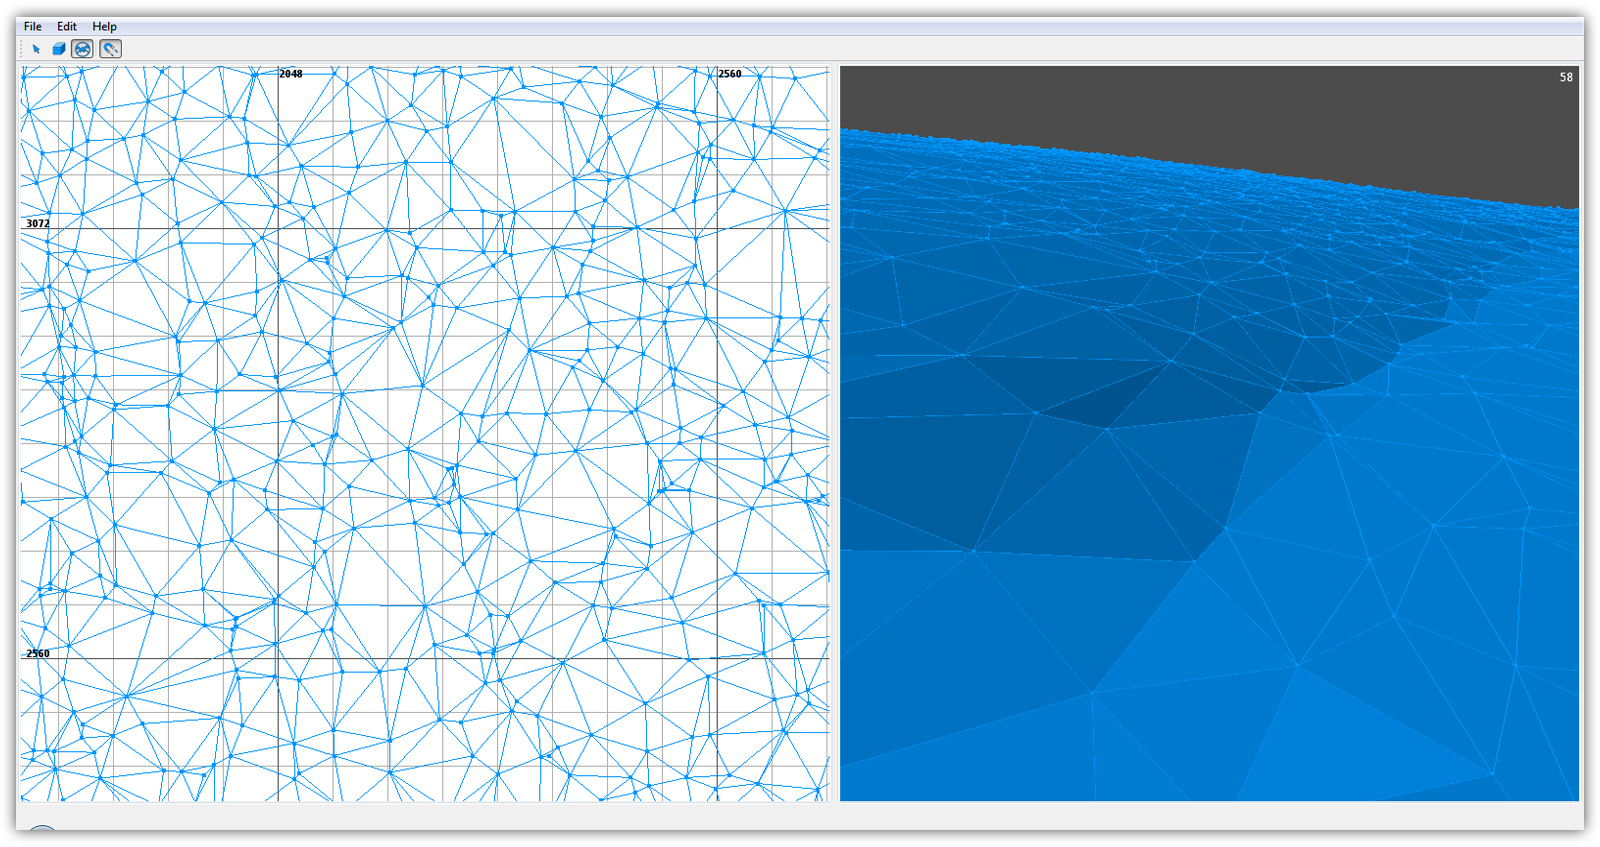
\includegraphics[width=\textwidth]{figures/currentstate-2}
	\caption{Our workbench animates incremental terrain mesh generation.} 
	\label{fig:currentstate}
\end{figure}

A \emph{geometric workbench} aids algorithm implementers and presenters by
providing facilities to dynamically visualize geometric algorithms. Implementers
can visually inspect geometric relationships and properties of data structures,
quickly recognizing erroneous computations. Presenters can produce
animations of their algorithms, more clearly conveying essential
ideas to their audience. Both types of geometers can interactively control the
flow of execution and easily generate degenerate input data.

\emph{Degree-driven algorithm design} encourages robust geometric computing by
attempting to minimize an algorithm's arithmetic precision with its running time
and space~\cite{millman2012degree}. Millman built a C++ library (DDAD) to
facilitate implementing algorithms with low-degree predicates. Our workbench
extends DDAD with a visual event system and provides a standalone GUI that can
generate input data and render algorithm execution.
Figure~\ref{fig:currentstate} captures the workbench rendering a terrain mesh
built by incremental delaunay triangulation.

This paper explains the benefits of using the DDAD workbench as a platform for
implementing and presenting degree-driven geometric algorithms. In
section~\ref{sec:taxonomy-previousworks-desiderata}, we define a taxonomy for
workbench systems and use it to place our workbench in the context of previous
works. We study Melkman's algorithm in section~\ref{sec:case-melkman} to show
how to leverage existing DDAD types to implement a simple 2-dimensional
algorithm. The inner workings of these types are revealed in
section~\ref{sec:workbench-architecture}. We conclude by studying incremental
Delaunay triangulation to show how to implement a complex 3-dimensional
algorithm.

% This paper provides a guided introduction to the inner workings of the DDAD
% workbench. It is intended for people interested in degree-driven algorithm
% design and who would like to use the DDAD library to get started implementing
% algorithms. We start out by explaining

%[todo: paragraph overviewing the paper]

% Section 2 reviews previous work. Section 3 recalls a general framework for
% designing software visualization systems. Section 4 uses the framework to
% explain our workbench desiderata. Section 5 provides an architectural overview
% of the workbench and section 6 runs through a case study of animating a convex
% hull algorithm. Section 7 concludes by explaining how current workbench
% architecture supports our desiderata and identifies areas in which it can
% improve.

 

\section{Taxonomy, Previous Works, and DDAD Desiderata}

% Taxonomies organize the properties of systems. Geometric workbench systems are a
% type of software visualization system. We define a taxonomy for workbench
% systems by synthesizing the specific elements of Dobkin's workbench
% taxonomy~\cite{hausner1999animation} with the broad categories of Price et.
% al.'s software visualization taxonomy~\cite{price1993principled}. we use
% the taxonomy to review previous workbench systems.

Taxonomies organize the properties of systems. This section defines a taxonomy
for geometric workbench systems, then uses the taxonomy to review previous
workbench systems and to organize the desired properties of the DDAD workbench
system.

% We define a taxonomy for workbench
% systems by synthesizing the specific elements of Dobkin's workbench taxonomy~\cite{hausner1999animation} with the broad categories of Price et.
% al.'s software visualization taxonomy~\cite{price1993principled}. we use
% the taxonomy to review previous workbench systems.  
% 
% A taxonomy is a means of organizing properties of a system. This section
% provides a taxonomy for geometric visualization systems, uses the taxonomy to
% guide a review of previous works, then uses the taxonomy to explain the desired
% properties of the DDAD workbench.

% From their thorough review of geometric workbench systems, Dobkin and Hausner
% extracted a set of design decisions that must be made by new
% systems~\cite{hausner1999animation}. However, a geometric workbench is a
% specific type of \emph{software visualization} (SV) system. The SV literature
% contains several well-developed taxonomies that are designed to evaluate SV
% systems~\cite{diehl2007software}. In particular, Price \emph{et al.} outline
% six major categories in which they judge SV systems: scope, content, form,
% method, interaction, and effectiveness~\cite{price1993principled}. We found
% that this detailed taxonomy provided a more structured way of organizing the
% desiderata of new workbench systems.
%  This section recalls the taxonomy for evaulating SV systems and relates each
% category to the specific case of workbench systems. The taxonomy is a
% hierarchy of categories, each of which may be described in terms of a question
% about the system. This makes the task of describing our specific desiderata
% quite easy because we may simply answer each of these questions in turn.

\subsection{Taxonomy} 

Geometric workbench systems are a type of software visualization system. Our
taxonomy synthesizes the specific elements of Dobkin's workbench
taxonomy~\cite{hausner1999animation} with the broad categories of Price et.
al.'s software visualization taxonomy~\cite{price1993principled}. It is composed
of five categories: scope, content, form, method, and interaction.

\paragraph{Scope.} What range of programs can the SV system take as input for
visualization? All geometric workbench systems specialize in visualizing
geometric algorithms, but each system makes different choices in regards to
scalability. Scalability refers to both input data and algorithm complexity. 

% \begin{enumerate}
%     \item Generality. Can the system handle a generalized range of programs or
%     does it display a fixed set of examples?
%     \begin{enumerate}
%       \item Hardware. What hardware does it run on?
%       \item Operating System. What operating system is required to run it?
%       \item Language. What programming language must user programs be written
%       in?
%       \begin{enumerate}
%         \item Concurrency. If the programming language is capable of
%         concurrency, can the SV system visualize the concurrent aspects?
%       \end{enumerate}
%       \item Applications. What are the restrictions on the kinds of user
%       programs that can be visualized?
%       \begin{enumerate}
%         \item Specialty. What kinds of programs is it particularly good at
%         visualizing (as opposed to simply capable of visualizing)?
%       \end{enumerate}
%     \end{enumerate}
%     \item Scalability. To what degree does the system scale up to handle large
%     examples?
%     \begin{enumerate}
%       \item Program. What is the largest program it can handle?
%       \item Data Sets. What is the largest input data set it can handle?
%     \end{enumerate}
%   \end{enumerate}

\paragraph{Content.} What information about the software can the SV system
visualize? In particular, systems may focus on visualizing the actual
implementation or the high level algorithm description. Often, these will
overlap, but sometimes visualizing implementation details clutters the
presentation of the high level algorithm.

% \begin{enumerate}
%     \item Program. To what degree does the system visualize the actual
%     implemented program? 
%     \begin{enumerate}
%       \item Code. To what degree does the system visualize the instructions in
%       the program source code?
%       \begin{enumerate}
%         \item Control Flow. To what degree does the system visualize the flow of
%         control in the program source code?
%       \end{enumerate}
%       \item Data. To what degree does the system visualize the data structures
%       in the program source code?
%       \begin{enumerate}
%         \item Data Flow. To what degree does the system visualize the flow of
%         data in the program source code?
%       \end{enumerate}
%     \end{enumerate}
%     \item Algorithm. To what degree does the system visualize the high-level
%     algorithm behind the software?
%     \begin{enumerate}
%       \item Instructions. To what degree does the system visualize the
%       instructions in the algorithm?
%       \begin{enumerate}
%         \item Control Flow. To what degree does the system visualize the flow of
%         control in the algorithm instructions?
%       \end{enumerate}
%       \item Data. To what degree does the system visualize the data structures
%       in the algorithm?
%       \begin{enumerate}
%         \item Data Flow. To what degree does the system visualize the flow of
%         data in the algorithm?
%       \end{enumerate}
%     \end{enumerate}
%     \item Fidelity and Completeness. Do the visual metaphors present the true
%     and complete behavior of the underlying virtual machine?
%     \begin{enumerate}
%       \item Invasiveness. If the system can be used to visual concurrent
%       applications, does its use disrupt the execution sequence of the program?
%     \end{enumerate}
%     \item Data Gathering Time. Is the data on which the visualization depends
%     gathered at compile-time, at run-time, or both?
%     \begin{enumerate}
%       \item Temporal Control Mapping. What is the mapping between 'program time'
%       and 'visualization time'?
%       \item Visualization Generation Time. Is the visualization produced as a
%       batch job (post-mortem) from data recorded during a previous run, or is it
%       produced live as the program executes?
%     \end{enumerate}
%   \end{enumerate}

\paragraph{Form.} What are the characteristics of the output of the system (the
visualization)? This category encompasses graphical vocabulary, granularity and
elision, and whether the system can present multiple views of the same data.
%   Oftentimes systems are structured around the model-view-controller
%   design pattern.

% \begin{enumerate}
%     \item Medium. What is the primary target medium for the visualization
%     system?
%     \item Presentation Style. What is the general appearance of the
%     visualization?
%     \begin{enumerate}
%       \item Graphical Vocabulary. What graphical elements are used in the
%       visualization produced by the system?
%       \begin{enumerate}
%         \item Colour. To what degree does the system make use of colour in its
%         visualizations?
%         \item Dimensions. To what degree are extra dimensions used in the
%         visualization?
%       \end{enumerate}
%       \item Animation. If the system gathers run-time data, to what degree does
%       the resulting visualization use animation?
%       \item Sound. To what degree does the system make use of sound to convey
%       information?
%     \end{enumerate}
%     \item Granularity. To what degree does the system present coarse-granularity
%     details?
%     \begin{enumerate}
%       \item Elision. To what degree does the system provide facilities for
%       eliding information?
%     \end{enumerate}
%     \item Multiple Views. To what degree can the system provide multiple
%     synchronized views of different parts of the software being visualized?
%     \item Program Synchronization. Can the system generate visualizations of
%     multiple programs simultaneously?
%   \end{enumerate}

\paragraph{Method.} How is the visualization specified? Automatic visualization
of algorithms is a difficult if not impossible task, so there is often a degree
of invasiveness. Systems may require users to annotate their code at visually
important points of execution.

% \begin{enumerate}
%     \item Visualization Specification Style. What style of specification is
%     used?
%     \begin{enumerate}
%       \item Intelligence. If the visualization is automatic, how advanced is the
%       visualization software from an AI point of view?
%       \item Tailorability. To what degree can the user customize the
%       visualization?
%       \begin{enumerate}
%         \item Customization Language. If the visualization is customizable, how
%         can the visualization be specified?
%       \end{enumerate}
%     \end{enumerate}
%     \item Connection Technique. How is the connection made between the
%     visualization and the actual software being visualized?
%     \begin{enumerate}
%       \item Code Ignorance Allowance. If the visualization system is not
%       completely automatic, how much knowledge of the program code is required
%       for a visualization to be produced for the user?
%       \item System-Code Coupling. How tightly is the visualization system
%       coupled with the code?
%     \end{enumerate}
%   \end{enumerate}

\paragraph{Interaction.} How does the user of the SV system interact with and
  control it? For geometric algorithm visualization, the user may need different
  camera types for 2 and 3 dimensions. For algorithm visualization in general,
  the user may want controls for speeding up, slowing down, pausing, resuming,
  and restarting algorithm execution. 

% \begin{enumerate}
%     \item Style. What method does the user employ to give instructions to the
%     system?
%     \item Navigation. To what degree does the system support navigation through
%     a visualization?
%     \begin{enumerate}
%       \item Elision Control. Can the user elide information or suppress detail
%       from the display?
%       \item Temporal Control. To what degree does the system allow the user to
%       control the temporal aspects of the execution of the program?
%       \begin{enumerate}
%         \item Direction. To what degree can the user reverse the temporal
%         direction of the visualization?
%         \item Speed. To what degree can the user control the speed of execution?
%       \end{enumerate}
%     \end{enumerate}
%     \item Scripting Facilities. Does the system provide facilities for managing
%     the recording and playing back of interactions with particular
%     visualizations?
%   \end{enumerate}

\subsection{Previous Works}

A geometric workbench combines a geometric algorithm library with a geometric
algorithm visualizer. \emph{Geometric algorithm libraries} provide a broad
selection of algorithms and the substrate of types upon which they are built.
\emph{Geometric algorithm visualizers} provide a GUI capable of animating and
visually debugging those algorithms implemented in the library. They borrow
heavily from techniques used in general algorithm animation
systems~\cite{brown1984system, stasko1990tango, stasko1995polka,
stasko1995samba}. Previous works may thus be categorized as
libraries~\cite{mehlhorn1989leda, fabri1998design, overmars1996designing,
fabri1996cgal}, visualizers~\cite{phillips1993geomview, hanson1994interactive,
amenta1995geomview, basken2002geowin}, and full workbench
systems~\cite{schorn1991robust, de1993geolab, de1993animation,
epstein1994workbench, tal1995visualization, shneerson1997gasp,
wei2009geobuilder}.

\paragraph{XYZ GeoBench.}

XYZ (eXperimental geometrY Zurich) GeoBench was a geometric workbench developed
by Peter Schorn under the supervision of Jurg Nievergelt. Schorn's 1991 thesis
focused on the question of how to produce good software for geometric
computation, with a particular emphasis on geometric
robustness~\cite{schorn1991robust}. Schorn describes the
GeoBench as ``a programming environment, implemented in an object oriented
language, for the rapid prototyping of geometric software and a testbed for
experiments,'' noting that ``algorithm animation is used for demonstration
purposes and debugging.'' The XYZ Library was built on top of the GeoBench and
offered implementations of a large number of geometric algorithms. 

There are several notable features about the GeoBench. The first is the use of
interchangable arithmetic and software simulation of parameterized floating
point numbers. In particular, algorithm implementations make reference to an
abstract 2D point class that does not specify a particular number system for the
coordinates. The abstract point class is extended to form concrete point types
for single-precision (realPoint), long integer (longIntPoint), and parameterized
floating point (floatPoint) coordinate types. Counterinuitively, the
parameterized floating point arithmetic was not used to ameliorate robustness
problems by increasing precision, rather it was used to simulate low precision
floating point to make the robustness problems more pronounced.

% The GeoBench had three major goals or desiderata. First was to be a programming
% environment. Provide the implementor of geometric algorithms with the necessary
% infrastructure for rapid prototyping. Ingredients of this environment include
% rich set of geometric primitives, fundamental set of basic geometric algorithms,
% collection of abstract data types and the ability to perform ``universal
% operations'' like input/output or scaling on geometric objects. Second was to be
% an interactive testbed for experiments. Wanted to measure an implementation's
% efficiency by comparing it to other programs solving the same problem. Would
% like to experiment with different implementations of abstract data structures
% and to try different models of arithmetic. Need to construct degenerate
% configurations as test cases and save them in a test suite. Third was algorithm
% animation. Most algos can be animated fairly easily since geometric objects have
% clear standard graphical representations. algo animation is used for
% demonstration in the classroom and for debugging.

\paragraph{Workbench.}

Workbench is a system similar to XYZ GeoBench that focused on implementing
complex geometric algorithms instead of robustness issues. The system is built
in Smalltalk and composed of three main components: a library, visualization
GUI, and tools for extending each. It focused heavily on empirical comparisons of different
algorithms and using animations for teaching and demonstration. They define the
minimum criteria for a geometric workbench as a system with: representations of
geometric objects, geometric data types, non-geometric data types, algorithmic
implementations that adhere to specification, different arithmetic types, and a
GUI that provides animation and debugging facilities.

% they identify two other projects (LEDA and GeoBench): LEDA had a large number of
% graph algorithms and well designed data types but was just then starting to move
% toward geometry, GeoBench is similar to workbench (UI + library) but main focus
% is on robust implementation of fundamental algorithms. the algorithmic portion
% of their software is layered with primitive operations and types on the bottom
% and more complex types on top. the ui component is separate and similarly
% layered. the primary goal of this project was to create a geometric computing
% environment: a tool for geometric computation applicable in a variety of
% contexts that provides useful facilities for dealing with the complex algorithms
% typical of computational geometry. they identify three main components such an
% environment must have: library of algs and data types, GUI for manipulating
% library objects, and tools for enhancing and extending the lib and GUI.
% empirical comparison of different algorithms and data structures is important,
% display and animation features are useful for teaching/demonstration. they
% consider the following worthwhile but didn't pursue them: optimizing
% implementations, handling degeneracies and numerical problems.
% 
% they define the minimum criteria for a geometry workbench as having:
% representations of geom objects (polygons etc), geometric data types/structures,
% nongeometric data types/structures (splay trees, heaps), algorithmic
% implementations adhering to specification, different arithmetic types, GUI with
% algorithm animation, programming environment and debugging facility (I/O of
% geometric objects). they implement the workbench in smalltalk

\paragraph{GeoLab.}

de Rezende created GeoLab, a system that binds together support for software and
algorithm development with realtime interaction~\cite{de1993geolab,
de1993animation}. The system supports software development with built-in
abstract data types for geometric objects, data structures, basic algorithms,
and mechanisms for incorporating new components \emph{without} recompilation.
The system supports user interaction with the ability to construct input data,
debug implementations visually, gather statistics, input/output geometric data,
and customize algorithm animations. Although the system is implemented in
object-oriented C++, algorithms are not necessarily member functions of the
classes upon which they operate -- they may be free functions. This echoes
Meyer's advice that minimal use of member functions can often increase
encapsulation.

% software
% development:
% build in ADT's for geometric types, data structures, basic algorithms and some
% complex geometric data structures, mechanisms for incorporation of new
% components WITHOUT recompilation of the environment, etc.
% support for interaction: GUI, ability to construct input data, debugging and
% statistics, I/O, customization of algorithm animation. written in C++.

% new modules are imported into the system via shared libraries, the kernel itself
% contains no geometric code. GUI consists of editing area, operation pallete,
% algorithms menu. random generators for input data. double hierarchy of classes -
% pure objects and graphics objects. for each pure geometric object (e.g. point2d)
% there is a graphical geometric counterpart. geometric algorithms are not
% necessarily methods of the classes they operate on - they may be free functions.

\paragraph{GASP.}

Tal and Dobkin describe the Geometric Animation System, Princeton
(GASP)~\cite{tal1995visualization}. The system allows users to quickly create 3D
visualizations, animate complex geometric algorithms, and visually debug
implementations. The use of style files to control the visual aspects of the
animation allows users to produce new renderings without recompiling the system.

% It can be used as an illustration tool for geometric
% constructions, to create videotapes to accompany talks, as a debugger, animator,
% and as an instructional aid to students. 

% three objectives set them apart from other
% animation systems such as Balsa Balsa-II Tango and Zeus: quick creation of 3d
% visulizations, can animate complex geometric algorithms, includes a visual
% debugging facility. the system may be used in many ways: illustration tool for
% constructions, videotapes to accompany talks/classes, for debugging, allow
% students to interact and experiment with animations, allows users to create
% animations to attach to their documents. previous systems identified two user
% types (client programmer and end user), they define three: end user, naive
% programmer (animations are easy), advanced programmer (can change the animation
% around). uses style files to control visual aspects of animations. thus, there
% are 4 parts to an animation: animation system, algorithm implementation, hooks
% to animation system inside implementation, style files. programmers concentrate
% on logical operations that need to be visualized (the what) but not how to do it
% (the how). identify four-dimensional space as future work.

%\paragraph{GASP-II (1998)}

%todo~\cite{shneerson1997gasp}.
% GASP-II had something to do with an electronic
% classroom~\cite{shneerson1997gasp}.

%\paragraph{WAVE (1999, 2001)}

%todo~\cite{baker1999visualizing, demetrescu2001visualizing}.

% tamassia and liotta got into visualizing geometric algorithms over the web in
% 1999 and 2001~\cite{baker1999visualizing, demetrescu2001visualizing}.

\paragraph{GeoBuilder.}

GeoBuilder is a cross-platform geometric workbench written in
Java~\cite{wei2009geobuilder}. It features a novel mechanism for automatically
positioning the 3D camera during algorithm execution and allows users to
collaborate on programming and visualization. Wei et al demonstrate the 3D
tracking feature by constructing convex hulls and detecting line segment
intersections. They note that automatically positioning a single view of an
algorithm may not be sufficient to capture all changes in algorithm state, and
identify automatic positioning of multiple cameras for future work.

% \subsection{Geometric algorithm libraries and visualizers}
% 
% \paragraph{LEDA}
% 
% The library of efficient data structures and algorithms (LEDA) is often
% mentioned in the context of workbenches.
% 
% \paragraph{CGAL}
% 
% The computational geometry algorithms library (CGAL) is the current standard
% implementation among the geometry community - it used to provide support for
% GeomView but now just has its own visualization module.

\paragraph{Geomview.}

Geomview is a geometric visualization system that focuses on rendering and
manipulating geometric data in 3-space~\cite{phillips1993geomview,
hanson1994interactive, amenta1995geomview}. It is able to render both static
geometry and dynamic geometry produced by an external program running
concurrently. External programs that use Geomview in this fashion are called
``external modules.'' It gained a large userbase after its initial release in 1991
due to its decoupled approach to animating geometric algorithms; users could
implement algorithms however they wanted and simply interface with Geomview at
runtime. Of particular note is its 4D visualization module that allow users to
explore 4-dimensional geometry through various projections. CGAL provides a
module for producing Geomview visualizations.

\paragraph{GeoWin.}

GeoWin is a C++ data type that provides the ability to visualize sets of
geometric objects, with a focus on two dimensions~\cite{basken2002geowin}. This
functionality may be used to visualize the output of geometric algorithms or to
animate the progression of algorithms. GeoWin defines a programming interface to
define scenes and an interactive interface to define how the user may interact
with the scene. The data type integrates directly with LEDA and CGAL while
custom libraries must implement the interfaces, entailing a dependency on LEDA
types.

\subsection{DDAD Desiderata}

Geometric objects on a digital computer are composed of two types of data:
numerical and combinatorial. Examples of numerical data include the
Cartesian coordinates of a point in 3-space, the length of a line segment
connecting two such points, or the angle between two such line segments.
Examples of combinatorial information include grouping two points as an
edge, grouping a collection of edges as a face, or grouping a collection of
faces as a surface.

Geometric algorithms that operate on geometric objects are best thought of as
two types of operations: predicates and constructions. Predicates determine
relationships between objects. A predicate might determine if a point is to
the left, right, or is collinear with a line segment, determine if a point is
inside, outside, or on a circle, or determine if a line intersects a plane in
one, none, or infinitely many points. Constructions produce new geometric
objects from existing geometric objects. A construction might produce the
rotation of a point around an origin, produce the point of intersection
between two line segments, or produce an offset of an algebraic curve.

\paragraph{Scope.} First, the system should visualize geometric algorithms
implemented with primitives and predicates from the degree-driven algorithm
design library (DDAD). Second, the system should provide example implementations
and visualizations of algorithms that solve textbook computational geometry
problems. Third, the system should be flexible enough to visualize new geometric
algorithms from the facilities used in example visualizations. Fourth, the
system should run well given inputs large enough to verify the correctness of a
particular implementation.

\paragraph{Content.} For algorithm implementers, the system should
visualize information about the concrete implementation of the algorithm. This
entails combining traditional debugging facilities with the new ability to
visualize geometric structures and operations. For algorithm presenters, the
system should visualize information about the high-level algorithm description.
This entails mechanisms for displaying visualizations that do not necessarily
correspond to the underlying implementation details.

\paragraph{Form.} First, the output medium should be an interactive computer
program. This is sufficient for implementers, but presenters may want to produce
a digital recording of an algorithm animation. Fortunately, screen capture
programs can facilitate producing this type of output. Second, the output should
have a rich graphical vocabulary, displaying standard graphics primitives
(points, lines, polygons), each with a variety of attributes (color,
transparency, pattern, texture). Presenters in particular desire highly
expressive output. Third, the output should contain both 2D and 3D elements.
The third dimension can be used both for visualizing inherently 3D algorithms
and to effectively display non-dimensional information. Fourth, the output
should have multiple levels of information granularity, with the ability to
elide and reveal specific levels as needed. Fifth, users should be able to view
the same data in multiple ways. This capability is particularly pertinent in
geometry where insight into a problem may be gained from viewing a dual
formulation (\emph{e.g.} viewing points as lines).

\paragraph{Method.} Implementers desire highly automated specifications that
minimally invade implementation source code. Increased automation increases the
likelihood a tool will be used for debugging assistance. Useful automated
visualizations require a high level of intelligence in order to correctly
recognize and display high level data structures. In contrast, presenters are
less concerned with automated visualization specifications, and accept a higher
degree of invasiveness in return for customization and increased expressibility.
The system should strike a balance between automation and customization.

\paragraph{Interaction.} First, users should be able to control the speed of
execution. This includes starting, stopping, speeding up, slowing down, and
single stepping. Second, users should be able to control a camera to navigate
around the scene and to focus on different objects. This is especially important
for 3D algorithms and larger data sets. Third, users should be able to record
and play back particular runs of a visualization. For presenters this could aid
pedagogy, and implementers might record when an algorithm fails.

% \subsection{Current Capabilities}
% 
% The workbench currently satisfies the desired functionality as follows. It
% extends the DDAD library with visual types and encapsulates these into a
% geometry kernel. The geometry kernel is paired with a visualizer that is capable
% of animating algorithm execution. The workbench strikes a balance between
% automated visualizations and expressive power by using object
% oriented design to encapsulate visual commands in lower level objects. The user
% is able to control the speed of execution and pause at important moments. They
% control two different views of the scene and can move these views interactively
% as the algorithm executes.


%==============================================================================
% @author Clinton Freeman <freeman@cs.unc.edu>
% @date 2014-05-23
%==============================================================================

\FloatBarrier
\section{Case Study: Melkman's Algorithm}

The DDAD workbench makes it easy for presenters and implementers to quickly
visualize new geometric objects and algorithms. In this section, we overview
using the workbench to implement and visualize Melkman's convex hull
algorithm~\cite{melkman1987line}. First, we implement the basic data
structures used by the algorithm and augment their methods with visualization
code. Second, we use these data structures to implement Melkman's algorithm. 
By visualizing the data structures in an object oriented way, we arrive at a
clean implementation of the algorithm.

% This section examines using our workbench to animate Melkman's convex hull
% algorithm~\cite{melkman1987line}. 

%==============================================================================

\subsection{Algorithm Overview}

A \emph{polyline} $P$ is a polygonal chain of vertices $p_1, p_2, \ldots, p_n$
connected by line segments $p_ip_{i+1}$ for $1 \leq i < n$. $P$ is \emph{simple}
if the only intersection between segments is at their shared endpoints.
Melkman's algorithm incrementally computes the convex hull of a simple polyline
in $O(n)$ time. 

The algorithm stores the hull's vertices in a doubly-ended queue (deque) and
maintains the invariant that they are stored in ccw order from head to tail,
starting and ending with the most recent vertex added to the hull. The algorithm
establishes the invariant initially by forming the deque with $p_2, p_1, p_2$ to
represent the convex hull of the first two points. 

Now, suppose we wish to add $p_i$ to the hull. Let $v, w$ be the vertices at the
tail of the deque and $u, v$ be the vertices at the head. Thus, $v$ is the most
recent vertex added to the hull, and we can speak of edges $uv$ and $vw$ as
being at the head and tail of the deque, respectively. 

If $p_i$ is not left of $uv$ or inside $uv$, then remove edge $uv$ from the
convex hull by popping the head of the deque; continue until $p_i$ is left of
the edge at the head. Similarly, if $p_i$ is not left of $vw$ or inside $vw$,
then remove edge $vw$ from the convex hull by popping the tail of the deque;
continue until $p_i$ is left of the edge at the tail. Finally, push $p_i$ onto
both the head and tail of the deque to restore the invariant.

On the other hand, if $p_i$ is left or inside both $uv$ and $vw$, then we can 
observe that $p_i$ is not on the convex hull: because the polyline from $v$ to
$p_i$ does not cross the polyline from $u$ to $v$ or from $v$ to $w$, $p_i$ can
leave the hull $CH(P_{i-1})$ only by crossing $uv$ or $vw$. Hull $CH(P_{i-1})$
is identical with $CH(P_i)$, and the invariant already holds.

%==============================================================================

\subsection{Data Structure Implementation}



The \texttt{Polyline\_2r} class uses a deque to store its vertices. The
\texttt{push\_back} and \texttt{pop\_back} methods are responsible for
visualizing how those operations affect the visual state of the object.

\lstinputlisting{code-samples/polyline.cpp}

\lstinputlisting{code-samples/polyline-push-back.cpp}

The \texttt{Polygon\_2r} class is composed of a \text{Polyline\_2r} boundary
that is responsible for visualizing vertices and edges. It can optionally
visualize the polygon interior by triangulating it into a fan.  

\lstinputlisting{code-samples/polygon.cpp}  
 
%==============================================================================

\subsection{Algorithm Implementation}

The code listed below shows the \texttt{Melkman} function which is our C++
implementation of Melkman's algorithm. The function takes as input a
\texttt{Polyline\_2r} and an \texttt{IGeometryObserver}, and produces as output
a \texttt{Polygon\_2r} object. All branching tests make use of the
\texttt{RIsLeftOrInsidePQ} predicate, which encapsulates the logic described in
the previous section. We will describe each of these in the paragraphs that
follow.
 
\lstinputlisting{code-samples/melkman.cpp} 

%==============================================================================
 
\subsection{Generating Input Data} 



%==============================================================================

% \begin{figure}[h]
% 	\centering
% 	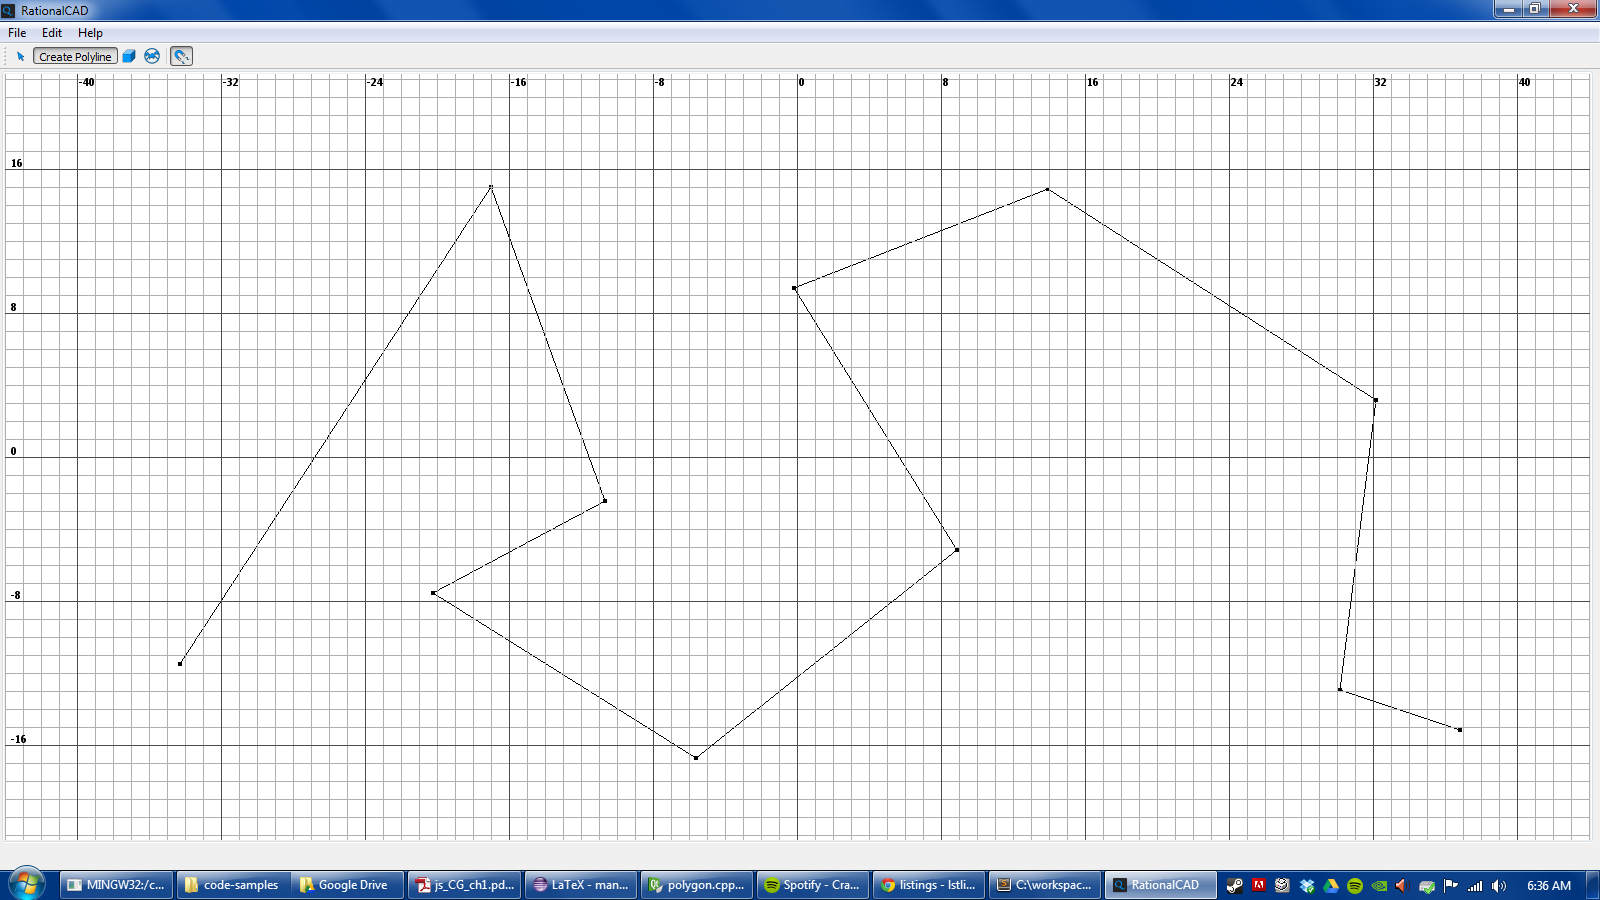
\includegraphics[width=\textwidth]{figures/melkman-input-1}
% 	\caption{Example polyline input.}
% 	\label{fig:melkman-input}
% \end{figure}

 
%As in Figure 1.18,

% Figure 1.19 continues the execution begun in Figure 1.16. It shows all of the
% deques and some of the hulls for $CH(P_5)$ through $CH(P_{14})$. Code is listed
% in Figure 1.20.

% It can also be used to compute the convex
% hull of arbitrary point sets if we first sort by $x$ coordinate, breaking ties
% by $y$ coordinate.

% Melkman's algorithm stores the convex hull vertices in a deque, or doubly-ended
% queue - a simple data structure that stores a list of elements and allows you to
% add and remove (by push() and pop()) elements from the front and back of the
% list. Melkman's algorithm maintains the invariant that the vertices of the
% convex hull CH(P\_i) are stored in a deque in ccw order from head to tail,
% starting and endign with the most recent vertex added to the hull.
% 
% Given an oriented line $pq$ and a point $r$, the 2D orientation predicate
% $\textsc{Orient2D}(p, q, r)$ answers the question, ``is $r$ to the left, right,
% or on $pq$?'' It is often written as the sign of the 2-by-2 determinant, $$
% \textsc{Orient2D}(p, q, r) = \textsc{Sign}\left( \begin{vmatrix} p_x-r_x &
% p_y-r_y \\ q_x-r_x & q_y-r_y \end{vmatrix} \right).$$

% Incremental convex hull algorithms construct the hull by examining each input
% point in turn, exploiting structure in the partial hull to help reduce
% computation. 
% Graham and Yao observed that if we know the points in advance, we
% may make our task easier by considering them in sorted order by $x$ coordinate,
% breaking ties by $y$ coordinate. Then point $p_i$ will always be a vertex of the
% convex hull $\text{CH}(P_i)$, and it will either be adjacent to $p_{i-1}$ or
% will cause $p_{i-1}$ to be removed from $\text{CH}(P_i)$.
 
% \begin{mdframed}[linecolor=white, backgroundcolor=algback, frametitle={Algorithm
% Melkman}] 
% \begin{algorithmic}[1]    
%     \Require Simple polyline $P = \langle v_1, \ldots, v_m \rangle$.
%     \Ensure $\text{CH}(P)$.
%     \vspace{0.75em}
%     \Procedure{Melkman}{$P$}
%     \State $H.push\_back(v_2); H.push\_back(v_1); H.push\_back(v_2);$
%     \Comment{Init hull}
%     \For{$i=3\ldots m$}
%     	\If{\textsc{!LeftOrInside}$(H.back(1), H.back(0), v_i)$ or
%     	\textsc{!LeftOrInside}$(v_i, H.front(1), H.front(0))$} 
%     		\While{\textsc{!LeftOrInside}$(H.back(1), H.back(0), v_i)$}
%     			\State $H.pop\_back();$
%     		\EndWhile
%     		\While{\textsc{!LeftOrInside}$(v_i, H.front(1), H.front(0))$}
%     			\State $H.pop\_front();$
%     		\EndWhile
%     		\State $H.push\_back(v_i);$
%     		\State $H.push\_front(v_i);$
%     	\EndIf
%     \EndFor
%     \State \Return $H$
%     \EndProcedure
% \end{algorithmic}
% \end{mdframed} 

% Animating an algorithm using the workbench is composed of a number of tasks,
% namely 
% \begin{itemize}
%   \item Implement input data structures and instrument them with visualization
%   code.
%   \item Optionally modify the GUI to allow the user to create instances of
%   the input data structure.
%   \item Implement output data structures and instrument them with visualization
%   code.
%   \item Implement predicates.
%   \item Implement the algorithm and instrument it with a small amount of
%   visualization code.
%   \item Optionally modify the GUI to allow the user to run the algorithm on
%   selected input data. 
% \end{itemize}

% \subsection{Data Structures}
% 
% polychain\_2r
% 
% polygon\_2r

% Animating any algorithm begins with generating the appropriate input. In the
% case of Melkman's algorithm, we begin by creating a simple polyline. This is
% accomplished by the user clicking on points in the 2D top-down orthographic
% view. The user may choose to place integer vertex coordinates or turn off
% snapping so that vertex coords are floating point or rational coords.
% 
% 
% 
% \begin{lstlisting}
% Polygon_2r Melkman(const PolyChain_2r& P, Visual::IGeometryObserver* ge_obs) {
%     Polygon_2r CH_P;
% 
% 
%     return CH_P;
% }
% \end{lstlisting}


\FloatBarrier
\section{Workbench Architecture}
\label{sec:workbench-architecture}

The workbench comprises two major components: a geometric algorithm library and
a geometric algorithm visualizer. The \emph{geometry library} implements
geometric algorithms. It defines types for arithmetic, linear algebra, and
geometric primitives (e.g. points, line segments, and triangles). These are
building blocks with which it defines more complex geometric objects (e.g.
polygons and polytopes). All of these may be used to implement geometric
algorithms. The \emph{visualizer} displays the execution of geometric
algorithms. It is structured using the model-view-controller (MVC) design
pattern. In particular, it maintains a visual model, several views of the visual
model, and a user interface that functions as the controller. In this section,
we are concerned with explaining how the library and visualizer work together to
produce algorithm visualizations.

\begin{figure}[htb]
\centering
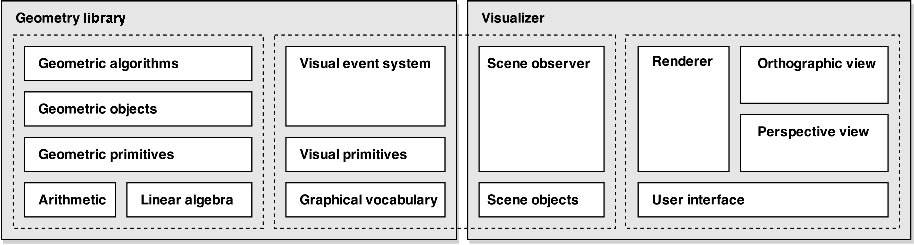
\includegraphics[width=\textwidth]{figures/components-uml-5} 
\caption{An abstract overview of the workbench architecture.}
\label{fig:components} 
\end{figure}

\subsection{The Geometry Library}

The \emph{arithmetic} and \emph{linear algebra} components are orthogonal to our
discussion of visualization. The \emph{graphical vocabulary} component is
necessary to define briefly but is straightforward to understand and depends
only on fundamental language types. In particular, it consists of types to
specify color, transparency, and a lighting model.

\emph{Geometric primitives} are geometric objects of constant size. We are
concerned with three: points, line segments, and triangles\footnote{Other
primitives include lines and rays but these are not directly supported by the
visual interface.}. Points are the basic unit of visualization. They are
equipped with unique identifiers (UIDs), assigned by registering with the visual
model. Line segments and triangles are combinatorial groupings of two and three
points, respectively. Thus, they are implicitly equipped with unique identifiers
given by the combinatorial grouping of their points' UIDs.

\emph{Visual primitives} are types that define the subset of graphical
vocabulary applicable to a corresponding geometric primitive. For
example, a visual point type might specify that points may be assigned a color
and rendered as either a circular or square sprite; a visual segment type might
also specify a color attribute but have no notion of a sprite shape.

The \emph{visual event system} defines the notion of observable geometry.
\emph{Observable geometry} objects notify their observers of changes in their
visual state by emitting signals. \emph{Geometry observers} handle these
notifications by implementing a corresponding slot. All higher level geometric
types that wish to be rendered by the visualizer must implement the observable
geometry interface. If a geometric object is composed of other observable
geometry objects, then it must also implement the geometry observer interface
and subscribe to those other objects.

Many geometric types will be composed of other observable geometry objects, so
we define an abstract base class that is both observable and capable of
observing other objects. By default, this base class forwards any visual events
it receives from the objects it observes onward to its own subscribers. In this
way, visual events are passed through a chain of event handlers, eventually
arriving at the scene observer in the visualizer.

\begin{figure}[htb]
\centering
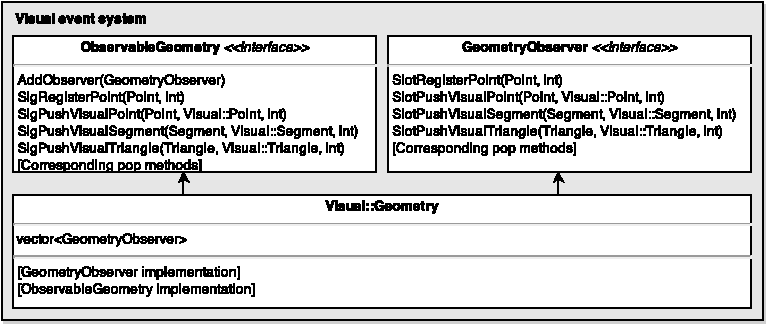
\includegraphics[width=\textwidth]{figures/visual-uml-6} 
\caption{The visual event system embedded in the geometry library.}
\label{fig:visual} 
\end{figure} 

\FloatBarrier
\subsection{The Visualizer}

\emph{Scene objects} are wrappers around geometric objects that implement an
interface required by the scene observer (e.g. being selectable or having a
name). Scene objects observe the geometric object they wrap, and may be observed
by the scene observer.

The \emph{scene observer} is the ultimate destination for all visual events
produced by geometric objects. It maintains three maps that pair unique
geometric primitives with a stack of visual primitives, the top of which defines
the current visual state. The scene observer is responsible for translating the
graphical vocabulary defined in the kernel into OpenGL buffer objects. The scene
observer lives inside of its own thread, and each of the visual events emitted
from an observable object may be given an integer value that will pause this
thread for a corresponding number of milliseconds.

The \emph{renderer} is responsible for managing OpenGL data and state.The
\emph{orthographic view} provides a top-down orthographic projection of the
scene. The user may pan around the plane and zoom in/zoom out. The
\emph{perspective view} provides a perspective projection of the scene. The user
may arbitrarily orient the camera and travel forward and backward along the view
direction.


%%==============================================================================
% @author Clinton Freeman <freeman@cs.unc.edu>
% @date 2014-12-28
%==============================================================================

\FloatBarrier
\section{Case Study: Gift Wrapping the Integer Hull}
\label{sec:case-ihull}

In this section, we use the workbench to implement and visualize gift wrapping
the integer hull of a convex polygon. The algorithm takes as input a
convex polygon $P$ and produces as output the convex hull of integer points
inside $P$. We conclude by using the GUI to generate an input polygon and run
the algorithm.

%==============================================================================

\subsection{Algorithm Overview}

In this section we first define invariants for identifying tangent ranges and
vertices of the integer hull and derive correct but slow code for maintaining
them. Next we derive the initialization and finalization.  Finally, we modify
the invariants and the code to compute the same sequence of hull vertices
faster, and analyze the running time.

Our input is a convex polygon, which can be represented as a counter-clockwise,
circular sequence of vertices and oriented supporting lines through the edges.
Our algorithms keep track of a single {\it current edge} with its support line 
$L$ that has the polygon to its left.  The current edge includes its ccw vertex,
denoted the {\it current vertex} $P$, but does not include the cw vertex.  The
operation $[P,L]=\op advance(P)$ advances to the next polygon vertex and line in
ccw order.

The output will be a ccw sequence of vertices of the integer hull, possibly with
a prefix of some additional vertices outside the integer hull.  As we will see
later, the precise statement is that the output is a sequence of vertices of the
integer hull of the region to the left of all polygon lines seen thus far---by
wrapping twice and discarding the prefix, we avoid specialized code for
initialization. 

% We begin with the invariants and body of a simple, but slow,
% algorithm~\ref{alg:slow} that identifies the sequence of integer hull vertices
% whose tangents lie in wedges on a stack.  It uses divide and conquer on wedges:
% either it identifies the hull vertex $z$ whose tangent range includes the entire
% wedge at the top of the stack, advancing to a new hull vertex if necessary,
% or it splits the wedge and stacks the pieces.
% 
% The number of invariants is almost larger than the number of lines of the
% algorithm, so let's start simply with the stack invariant.
% \begin{lemma}\label{lem:stack}
% The stack contains wedges defined by pairs of integer vectors $u$,$v$ that
% form unit area parallelograms that are consecutive in ccw order top to
% bottom, provided that this is true initially.
% \end{lemma}
% \begin{proof} 
% Suppose that wedge $[u,v)$ is popped in line~\ref{a1:pop}; if nothing is pushed,
% the invariant holds.  Parallelogram $uv$ has unit area, so $\determ{u.x&u.y\\
% v.x&v.y}=1$.  By row operations $\determ{u.x&u.y\\ u.x+v.x&u.y+v.y}=1$, so
% parallelogram $u,u{+}v$ also has unit area, as does $u{+}v,v$.  These are pushed
% onto the stack (line~\ref{a1:push}) in an order that preserves the invariant.
% \end{proof}
%  
% \begin{algorithm}[ht]
%   \begin{minipage}{\algwidth}\hrule\medskip
% Input: 
% $S$, a stack of wedges defined by pairs of integer vectors $u$,$v$ that
% form unit area parallelograms. From top to bottom the wedges are
% consecutive in ccw order. \\
% $P$,$L$ the current vertex and line of a convex polygon, and\\
% $z$, a vertex of the integer hull with a supporting line direction in the top wedge
% $u$,$v$ and with segment $\seg{z,u}$ crossing the current polygon edge.\\
% Output: The sequence of integer hull vertices whose tangent ranges
% cover the wedges on the stack. 
%  \smallskip
% \begin{alg}%
% proc \op ProcessWedge(S,z, P,L)\+\\
% \kw{while} stack $S$ is not empty\+\\
% $[u,v)=\op pop(S)$;\label{a1:pop}\\
% \kw{if} $L$ parallels or intersects \ray{z,v}\+\\
% \kw{while} $P$ is right of \ray{z,v} \label{a1:advP}\+\\
% $[P,L]=\op advance(P)$;\\
% \kw{if} $z$ right of $L$, return $\emptyset$; \kw{endif} \label{a1:test}\-\\
% \kw{endwhile}\\
% $z=\op lastBefore(z,v,L)$;\label{a1:z}\-\\
% \kw{else} split wedge\+\\
% \op push([u+v,v),S);\label{a1:push}\\
% \op push([u,u+v),S);\-\\
% \kw{endif}\-\\
% \kw{endwhile}\>\>\>\>\>\>\>\qquad\smash{\includegraphics[scale=.9]{figs/wedge}}\stepcounter{figure}
% \end{alg}\medskip\hrule
% \end{minipage}
% \caption{We either find that the
%   tangent range of $z$ covers the rest of the wedge, and possibly
%   identifies the next integer hull vertex ccw,  or we split the wedge}
% \label{alg:slow}
% \end{algorithm}
% 
% 
% Let $z$ be an integer point that satisfies three conditions with
% respect to the wedge $[u,v)$ and current edge of the convex polygon defining the hull 
% \begin{enumerate}[noitemsep]
% \item $z$ has a supporting line direction $\tau$ that lies in wedge
% $[u,v)$.
% \item \seg{z,z{+}u} intersects the current polygon edge, and
% \item $z$  lies on or to the left of all polygon lines seen so far.
% \end{enumerate}
% 
% \begin{lemma}
% Algorithm~\ref{alg:slow} maintains the conditions on $z$ and the
% current polygon edge, or reveals that the polygon contains no grid
% points. 
% \end{lemma}
% \begin{proof}
% Suppose first that the algorithm reaches
% line~\ref{a1:advP} because current polygon line $L$ intersects
% \ray{z,v}.  The polygon boundary from $\ray{z,u}$ to $\ray{z,v}$
% remains inside a sequence of unit parallelograms in direction
% $v$,  as seen in the figure with Algorithm~\ref{alg:slow}.   We
% advance $P$ until the current edge intersects \ray{z,v}.  
% 
% In the process of advancing, if we find $z$ to the right of the
% current polygon line $L$, then the entire polygon must lie on and to
% the left of $L$, support line $\tau$, and the boundary from $u$ to
% $\ray{z,v}$.  Since this is entirely contained in the unit
% parallelograms, the polygon contains no integer points, and we return
% and report that.  
% 
% In the usual case, by line~\ref{a1:z} we will have verified that $z$ remains left or on all lines
% that we advanced over, and we can find the last integer point on
% \ray{z,v} inside the  polygon, and call it $z$.  Whether this is a new
% $z$ or the old $z$, the current edge of the polygon intersects
% $\seg{z,v}$, which will become $\seg{z,u}$ after the next pop, by the
% stack invariant of Lemma~\ref{lem:stack}. Also, there will be a
% support line just ccw of $v$ which will serve as~$\tau$.
% 
% On the other hand, if algorithm reaches
% line~\ref{a1:push} then the only concern is if the  support line
% $\tau$ does not lie in the top wedge $u,u{+}v$ because it lies in
% $u{+}v,v$ instead.  But that can happen only if $z+u{+}v$ does not lie
% inside the polygon, so the top wedge will be popped on the next
% iteration.  (We could have handled this by pushing only if needed, but
% that will happen in the next algorithm.)
% 
% Thus, the conditions on $z$, the current edge of the polygon, and top
% wedge are invariant. 
% \end{proof}
% 
% 
% \subsection{Initialization and finalization}
% To initialize Algorithm~\ref{alg:slow}, we 
% push onto the stack six quadrants, in order II,I,IV,III,II,I, so I is
% on top with $u=(1,0)$ and $v=(0,1)$.  We choose coordinates for $z$
% as floor of the maximum $x$ and minimum $y$ coordinates of the
% polygon, and let the current $P$ be the vertex with max $x$
% coordinate and create an initial line $L$ parallel to the $y$ axis
% through $P$.  These choices satisfy all the invariants. 
% 
% We claim that this algorithm does terminate; it cannot keep filling the stack without advancing $P$. 
% Consider a wedge $[u,v)$ for which $L$ does not cross \ray{z,v}.  Note that this puts $P$ right of \ray{z,v}.  
% Since $L$ does separate $z$ from $z+u$, $L$ and \ray{zP} define a non-empty angle range around $P$.
% Split the wedge and consider whether $u+v$ lies cw, in, or ccw of this range: if cw, we continue in $[u,u{+}v)$, if ccw, we push and pop $[u,u{+}v)$  and continue in $[u{+}v, v)$.  In both cases this is the range containing $P$ in the interior.  Because the wedge narrows, we eventually  find $u+v$ in the range between $L$ and \ray{zP}, continuing in a wedge containing $P$ in the interior, so we advance $P$.   
% 
% Note from this argument that  rather than coarser parameters like 
% It is tempting to try use $n$, the number of vertices of
% the input polygon, and $d$, its diameter, to establish a coarse bound
% of $O(n+d)$, but the argument shows that the number of times a wedge is split 
% depends on the detailed geometry of the input, like the slope of polygon line $L$.
% in fact, splitting can generate vectors that extend  far beyond the polygon if
% the precision of the coordinates defining $L$ is sufficiently high.
% This is one of the problems that we will solve in the next subsection.
% 
% We mentioned that this initialization can generate a prefix of integer
% points 
% that lie outside the final integer hull. Our initial $z$ certainly
% does, since it is outside the polygon.  The next point may also,
% because if we split the polygon into upper and lower chains at the
% vertices that are extreme in $x$, then we advance $P$ on the upper
% chain to cross \ray{z,v} and take the highest grid point below the
% upper chain as our new $z$.  But this $z$ may also be below the lower chain; a
% thin polygon 
% may contain no integer points at this $x$ coordinate.  Our $z$ is
% known to be inside only those lines that have been seen.  When we
% complete quadrant II and pop III, however, we have seen all upper lines, and all
% lower lines relevant to determining the integer hull vertex with minimum
% $x$ coordinate, breaking ties by min $y$.  We can then discard all
% preceding vertices and continue.  When we complete II for the second
% time, we have returned to the same vertex and completed the integer
% hull.   We summarize in the following theorem.
% \begin{theorem}
% Algorithm~\ref{alg:slow} computes the vertices of the integer hull
% inside the given convex polygon.
% \end{theorem}
% 
% \subsection{Wrapping the integer hull efficiently}
% 
% Algorithm~\ref{alg:slow} can be slow for two reasons.  The first is
% subtle, but was already mentioned: since $L$'s
% slope comes from the input polygon unnecessary refinement may be
% needed to find a ray \ray{z,v} that intersects line $L$.  
% The second is the reason
% that Euclid's subtractive GCD computation can be slow:  If we
% alternate between replacing $u$ or $v$ with $u+v$, then vector length
% grows exponentially, but if we update just one, then length grows
% linearly.  Just as we
% would prefer to divide instead of performing repeated subtraction for GCD, we
% would prefer to multiply instead of performing repeated addition to find the next wedge. 
% 
% 
% Figure~\ref{fig:wedge2} copies the parallelogram $uv$ in both the $u$ and $v$ directions, and considers how the polygon boundary can next exit this {\it extended wedge}. Let $z'=z+u+v$.
% \smallbreak\noindent{\bf A:\/} The polygon could reach segment \seg{z,v}, with $z$ continuing to be the integer hull vertex whose tangent range we are finding, as in Alg.~\ref{alg:slow}.
% \smallbreak\noindent{\bf B:\/}   The polygon could reach ray
% \ray{z,v}, completing the tangent range for $z$, and beginning one for new hull vertex $z$,
% as in Alg.~\ref{alg:slow}.
% \smallbreak\noindent{\bf C:\/}  The polygon could reach ray \ray{z',v}, which corresponds to repeating $[u,v)\to [u{+}v,v)$ by repeated
% splits and pops in Alg.~\ref{alg:slow}.  We update $u=\op lastBefore(z',v,L)-z$, jumping straight to the outcome of the repeated splits and pops.
% \smallbreak\noindent{\bf D:\/}  The polygon could reach ray \ray{z',u}, which corresponds to repeated splitting $[u,v)\to [u,u{+}v)$ in Alg.~\ref{alg:slow}.
% We update $v=\op lastBefore(z',u,L)-z$, but need to change the  invariants since we don't want to push all the $[u{+}v,v)$ wedges that we skip over.  
% 
% \figbox[l]{\includegraphics[width=.5\textwidth]{figs/wedge2}}{figure}{fig:wedge2}{Exiting $uv$ parallelograms in Alg.~\ref{alg:fast}}
% \smallbreak\noindent{\bf E:\/}  The polygon line could have $z$ to the right, in which case the polygon contains no grid points as in Alg.~\ref{alg:slow}.
% 
% 
% Case D necessitates the following invariant changes.  Before updating
% $v$, in line~\ref{a2:D} we push $[u,v)$ to represent all wedges
%   $[iu+v,(i+1)u+v)$, which is just the area covered by copying the
%     parallelogram $uv$ in direction $u$.  Thus, the stacked wedges may
%     be nested or consecutive, but they will be in ccw order by $v$.
%     Since popping a wedge may give a containing wedge, we no longer
%     know that \seg{z,u} intersects the current polygon edge, but we do
%     know that it intersected the polygon at the time it was pushed,
%     and that the current edge has a point inside the wedge.  With
%     these invariant changes, we can show that Alg.~\ref{alg:fast}
%     identifies the same vertices as Alg.~\ref{alg:slow}, so with the
%     same initialization and finalization it computes the integer hull.
% 
% \begin{theorem}
%   Given an $n$-vertex convex polygon of diameter $d$ with single
%   precision coordinates, Algorithm~\ref{alg:fast} computes the
%   $m$-vertex integer hull in $O(n+m\log d)$ steps and double
%   precision. Space required is $O(\log d)$.
% \end{theorem}
% \begin{proof}
% Advancing $P$ takes $O(n)$ time, since we go around less than twice.
% Cases C and D alternate until terminated by Case A, B, or E. Case E
% can happen only once; B only $m$ times.  Since C takes $O(1)$ time and
% does not increase stack height, we fold it into the case that follows.
% Each string of C/D terminates with a case B, creating a new vertex of
% the integer hull, or E; the vectors grow at least as large as the
% Fibonacci numbers~\cite{davenport1999higher}, and so have at most
% $\log_\phi d$ alternations for the new edge, where $\phi=(1+\sqrt
% 5)/2$ is the golden ratio.  Since case D is the only case that pushes
% more than one item onto the stack after initialization, the stack
% depth is $\log_\phi d$, and the total number of wedges stacked is
% $m\log_\phi d$.  This also bounds the number of wedges popped by
% $A$.
% \end{proof}
% With a little more work and Jensen's inequality, we can express the
% time bound as $O(n+m\log (d/m))$, but since $m=O(d^{2/3})$ (Har-Peled
% has a short proof~\cite{har1998output}) this would not be an
% asymptotic improvement.  The same worst-case time bound can be
% achieved by a constant-space algorithm -- rather than stacking the
% wedges, we could start from a quadrant and work forward each time.
% Our preliminary experiments suggest that stacking is faster; we will
% include a brief experimental section in the next version of the paper.
% 
% 
% \begin{algorithm}[htp]
%   \begin{minipage}{\algwidth}\hrule\medskip
% Input: 
% $S$, a stack of wedges defined by pairs of integer vectors $u$,$v$ that
% form unit area parallelograms. From top to bottom the wedges are
%  in ccw order by $v$ and consecutive wedges are either adjacent or nested. \\
% $z$, an integer point, left or on all polygon lines seen so far, with a tangent in the top wedge
% $u$,$v$, with segment $\seg{z,u}$ crossing the polygon.\\
% $P$,$L$ the current vertex and line of a convex polygon, for which
%  some point of the current edge is right of \ray{z,v} and \ray{z{+}v,u}.\\
% Output: The sequence of integer hull vertices whose tangent ranges
% cover the wedges on the stack. 
%  \smallskip
% \begin{alg}%
% proc \op ProcessWedges(S,z,P,L)\+\\
% \kw{while} stack $S$ is not empty\+\\
% $[u,v)=\op pop(S)$;\label{a2:pop}\\
% \kw{while} $P$ is right of \ray{z,v} and \ray{z{+}v,u}\+\\
% $[P,L]=\op advance(P)$;\label{a2:advP}\\
% \kw{if} $z$ right of $L$, return $\emptyset$; \kw{endif} \-\\
% \kw{endwhile}\\
% \kw{if} $z+u$ is not right of $L$ \label{a2:A}// if not Case A\+\\
% \kw{if} $z+u+v$ is not right of $L$\+\\
% \op push([u,v),S); \label{a2:D}// Case D: in $u$ direction\\
% $v=\op lastBefore(z{+}v,u,L)-z$;\\
% \op push([u,v),S);\-\\
% \kw{else} // in $v$ direction\+\\
% \kw{while} $P$ is right of \ray{z,v} and left of \ray{z{+}u,v}\label{a2:while2}\+\\
% $[P,L]=\op advance(P)$;\label{a2:advP2}\\
% \kw{if} $z$ right of $L$, return $\emptyset$; \kw{endif} \-\\
% \kw{endwhile}\\
% \kw{if} $P$ is not right of \ray{z,v}  // Case B (or A): end wedge\+\\
% $z=\op lastBefore(z,v,L)$; \label{a2:B}// new (or same) vertex\-\\
% \kw{else} // Case C:  \+\\
% $u=\op lastBefore(z{+}u,v,L)-z$;\label{a2:C}\\
% \op push([u,v),S);\-\\
% \kw{endif}\-\\
% \kw{endif}\-\\
% \kw{endif}\-\\
% \kw{endwhile}
% \end{alg}\medskip\hrule
% \end{minipage}
% \caption{Faster processing for the same hull vertices}
% \label{alg:fast}
% \end{algorithm}

%==============================================================================

\subsection{Algorithm Implementation}

%==============================================================================

\subsection{Generating Input Data and Executing IHull} 


%==============================================================================
% @author Clinton Freeman <freeman@cs.unc.edu>
% @date 2014-11-26
%==============================================================================

\FloatBarrier
\section{Case Study: Incremental Delaunay Triangulation}
\label{sec:case-delaunay}

In this section, we use the workbench to implement and visualize an incremental
Delaunay triangulation algorithm~\cite{lischinski1994incremental}. The algorithm
takes as input a point set and produces as output a triangulation that is
\emph{Delaunay}: the circumcircle of any triangle in the triangulation does not
contain any input points in its interior. Our workbench already has these types
implemented, complete with visualization code for each basic operation.
After explaining how the algorithm works, we introduce the quad-edge data
structure and use it to arrive at a correct implementation. We conclude by using
the GUI to generate an input point set and run the algorithm. 

%==============================================================================

\subsection{Algorithm Overview}

The algorithm starts with a triangle large enough to contain all input points,
and adds points into the triangulation one by one, maintaining the invariant
that the triangulation is Delaunay. Figure 2 illustrates the point insertion
process. First, the triangle containing the new point $p$ is located (2a). New
edges are created to connect $p$ to the vertices of the containing triangle
(2b). The old edges of the triangle are inspected to verify that they still
satisfy the empty circumcircle condition. If the condition is satisfied (2c) the
edge remains unchanged. If it is violated (2d) the offending edge is flipped,
that is, replaced by the other diagonal of the surrounding quadrilateral. In
this case two more edges become candidates for inspection (edges $a$ and $b$ in
Figure 2e.) The process continues until no more candidates remain, resulting in
the triangulation shown in Figure 2f.

% In the worst case the insertion of a point can require $O(n)$ edges to be
% flipped. However, in practice the average number of edges tested per insertion
% is small (< 9). Guibas, Knuth, and Sharir have shown that if the insertion order is
% randomized, the expected time is O(1) per insertion (Guibas et al. 1990).

Locating the containing triangle can be done in an optimal $O(\log n)$ time, but
this requires maintaining complicated data structures. Alternatively, the
triangle can be located by starting from an arbitrary place in the triangulation
and moving in the direction of $p$ until the containing triangle is reached.
This requires $O(n)$ time, but if the inserted points are uniformly distributed,
the expected number of operations to locate a point is only $O(n^{1/2})$. A
simple improvement is to always resume the search from the triangle that was
found last: in this way, when the points to be located are near each other, the
containing triangles are determined quickly.

% Figure 3 shows the DT and the corresponding VD produced by this algorithm from
% 250 random points in the unit square. Note that because the quad-edge data
% structure represents both the triangulation and its dual, the topology of the
% Voronoi diagram is readily available from the DT constructed by the algorithm.
% To have a complete VD one only needs to compute the circumcenters of all the
% triangles (i.e., the locations of the Voronoi vertices.)

% A \emph{polyline} $P$ is a polygonal chain of vertices $p_1, p_2, \ldots, p_n$
% connected by line segments $\seg{p_ip_{i+1}}$ for $1 \leq i < n$. $P$ is
% \emph{simple} if the only intersection between segments is at their shared endpoints.
% Melkman's algorithm incrementally computes the convex hull of a simple polyline
% in $O(n)$ time. 
% 
% The algorithm stores the hull's vertices in a doubly-ended queue (deque) and
% maintains the invariant that they are stored in ccw order from head to tail,
% starting and ending with the most recent vertex added to the hull. The algorithm
% establishes the invariant initially by forming the deque with $p_2, p_1, p_2$ to
% represent the convex hull of the first two points. 
% 
% Now, suppose we wish to add $p_i$ to the hull. Let $v, w$ be the vertices at the
% tail of the deque and $u, v$ be the vertices at the head. Thus, $v$ is the most
% recent vertex added to the hull, and we can speak of edges $\seg{uv}$ and
% $\seg{vw}$ as being at the head and tail of the deque, respectively. 
% 
% If $p_i$ is not left of $\seg{uv}$ or inside $\seg{uv}$, then remove edge
% $\seg{uv}$ from the convex hull by popping the head of the deque; continue until
% $p_i$ is left of the edge at the head. Similarly, if $p_i$ is not left of
% $\seg{vw}$ or inside $\seg{vw}$, then remove edge $\seg{vw}$ from the convex
% hull by popping the tail of the deque; continue until $p_i$ is left of the edge
% at the tail. Finally, push $p_i$ onto both the head and tail of the deque to
% restore the invariant.
% 
% On the other hand, if $p_i$ is left or inside both $\seg{uv}$ and $\seg{vw}$,
% then we can observe that $p_i$ is not on the convex hull: because the polyline
% from $v$ to $p_i$ does not cross the polyline from $u$ to $v$ or from $v$ to
% $w$, $p_i$ can leave the hull $CH(P_{i-1})$ only by crossing $\seg{uv}$ or
% $\seg{vw}$. Hull $CH(P_{i-1})$ is identical with $CH(P_i)$, and the invariant
% already holds.

%==============================================================================

\subsection{Algorithm Implementation}

The incremental DT algorithm involves one geometric object (a subdivision), and
requires a single degree-four predicate to check whether a point is in, on, or
outside the circle defined by three points. The DDAD workbench provides the
geometric type (\texttt{Subdivision\_2r}) and the predicate
(\texttt{InCircle\_2r}). 

The quad-edge data structure (Guibas and Stolfi 1985) was designed for
representing general subdivisions of orientable manifolds. It is similar to the
winged-edge data structure (Baumgart 1975), but it simultaneously represents
both the subdivision and its dual. Each quad-edge record groups together four
directed edges corresponding to a single undirected edge in the subdivision and
to its dual edge (Figure 1a). Each directed edge has two pointers: a next
pointer to the next counterclockwise edge around its origin, and a data pointer
to geometrical and other nontopological information (such as the coordinates of
its origin.) 

Figures 1b and 1c illustrate how three edges incident on the same
vertex are represented using the quad-edge data structure: the vertex itself
corresponds to the inner cycle of pointers in Figure 1c. The remaining three
cycles correspond to the three faces meeting at the vertex.

Aside from a primitive to create an edge (MakeEdge), a single topological
operator Splice is defined that can be used to link disjoint edges together as
well as to break two linked edges apart. This operator is its own inverse and
together with MakeEdge it can be used to construct any subdivision.

% Melkman's algorithm involves two geometric objects (polylines and polygons), and
% requires only a single degree-two predicate to check whether a point is to the
% left or inside of a directed line segment. The DDAD workbench provides both
% geometric types (\texttt{Polyline\_2r} and \texttt{Polygon\_2r}), and the
% predicate \texttt{RIsLeftOfOrInsidePQ}. Both geometric types are built using a
% deque as an underlying data store, so we will have the push and pop
% capabilities we need. All two dimensional geometric types are given methods to
% set the $z$ coordinate (or \emph{z-order}) of all its vertices so that users can
% draw some objects above or below others. 
% 
% The final type we must use is \texttt{IGeometryObserver}. All DDAD geometric
% types are built to be observed by other types that implement the
% \texttt{IGeometryObserver} interface. Geometric algorithm implementations that
% wish to be visualized will usually be a free function with an
% \texttt{IGeometryObserver} as the last input argument. The only thing we need to
% do with the \texttt{observer} is to have it observe the output polygon before we
% perform any operations it.
% 
% Code listing~\ref{melkman-function} shows \texttt{Melkman}, the final 
% implementation of Melkman's algorithm. The function takes as input a 
% \texttt{Polyline\_2r} and an \texttt{IGeometryObserver}, and produces as output
% a \texttt{Polygon\_2r} object. All branching tests make use of the
% \texttt{RIsLeftOrInsidePQ} predicate. Aside from a few lines setting up colors,
% z-order, and observing the output hull, the implementation is a straightforward
% transcription of the algorithm, uncluttered by visualization code. Of course,
% the visualization code must exist somewhere; we cover the high level mechanics
% in section~\ref{sec:workbench-architecture} and the specific details of the
% polyline and polygon types in section~\ref{sec:polyline-polygon}.
%  
% \lstinputlisting[float,caption=Melkman
% implementation,label=melkman-function]{code-samples/melkman.cpp}

%==============================================================================

\subsection{Generating Input Data and Executing Incremental Delaunay} 

% The workbench GUI is composed of a toolbar and two views: orthographic and
% perspective. The toolbar contains input buttons and a button for turning
% snapping on and off. The orthographic view contains an integer grid and allows
% the user to zoom and pan the camera. The perspective view renders the scene in
% 3D and allows the user to move and rotate the camera.
% 
% \begin{figure}[htb]
% 	\centering
% 	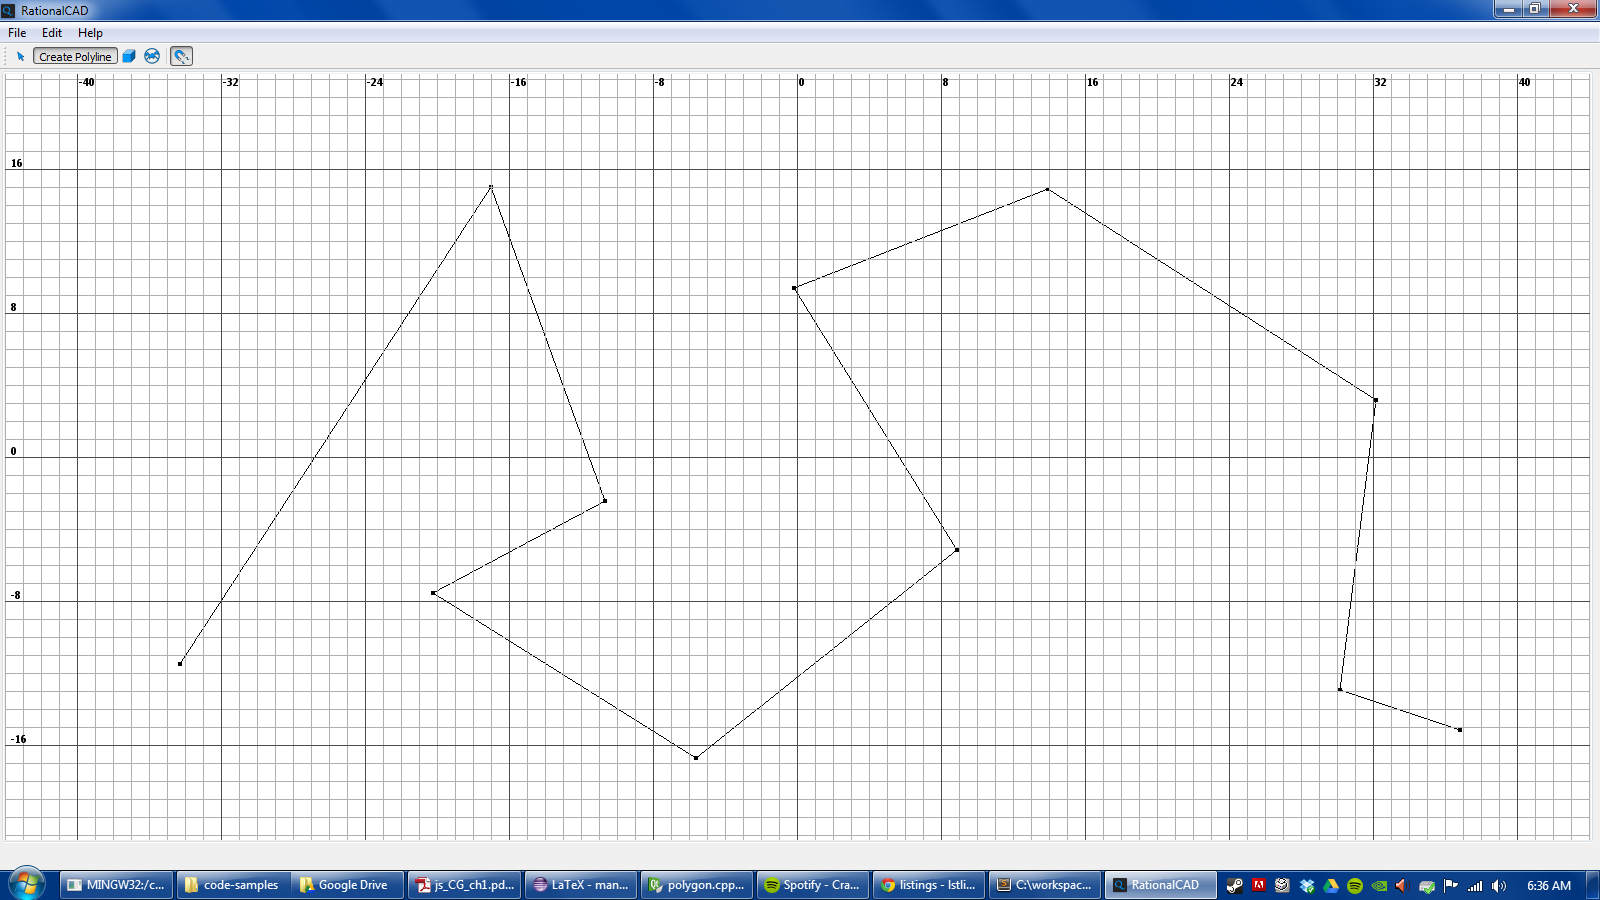
\includegraphics[width=\textwidth]{figures/melkman-input-1}
% 	\caption{Input polyline with Melkman listed in the context menu.} 
% 	\label{fig:melkman-input}
% \end{figure}
% 
% \begin{figure}[htb]
% 	\centering
% 	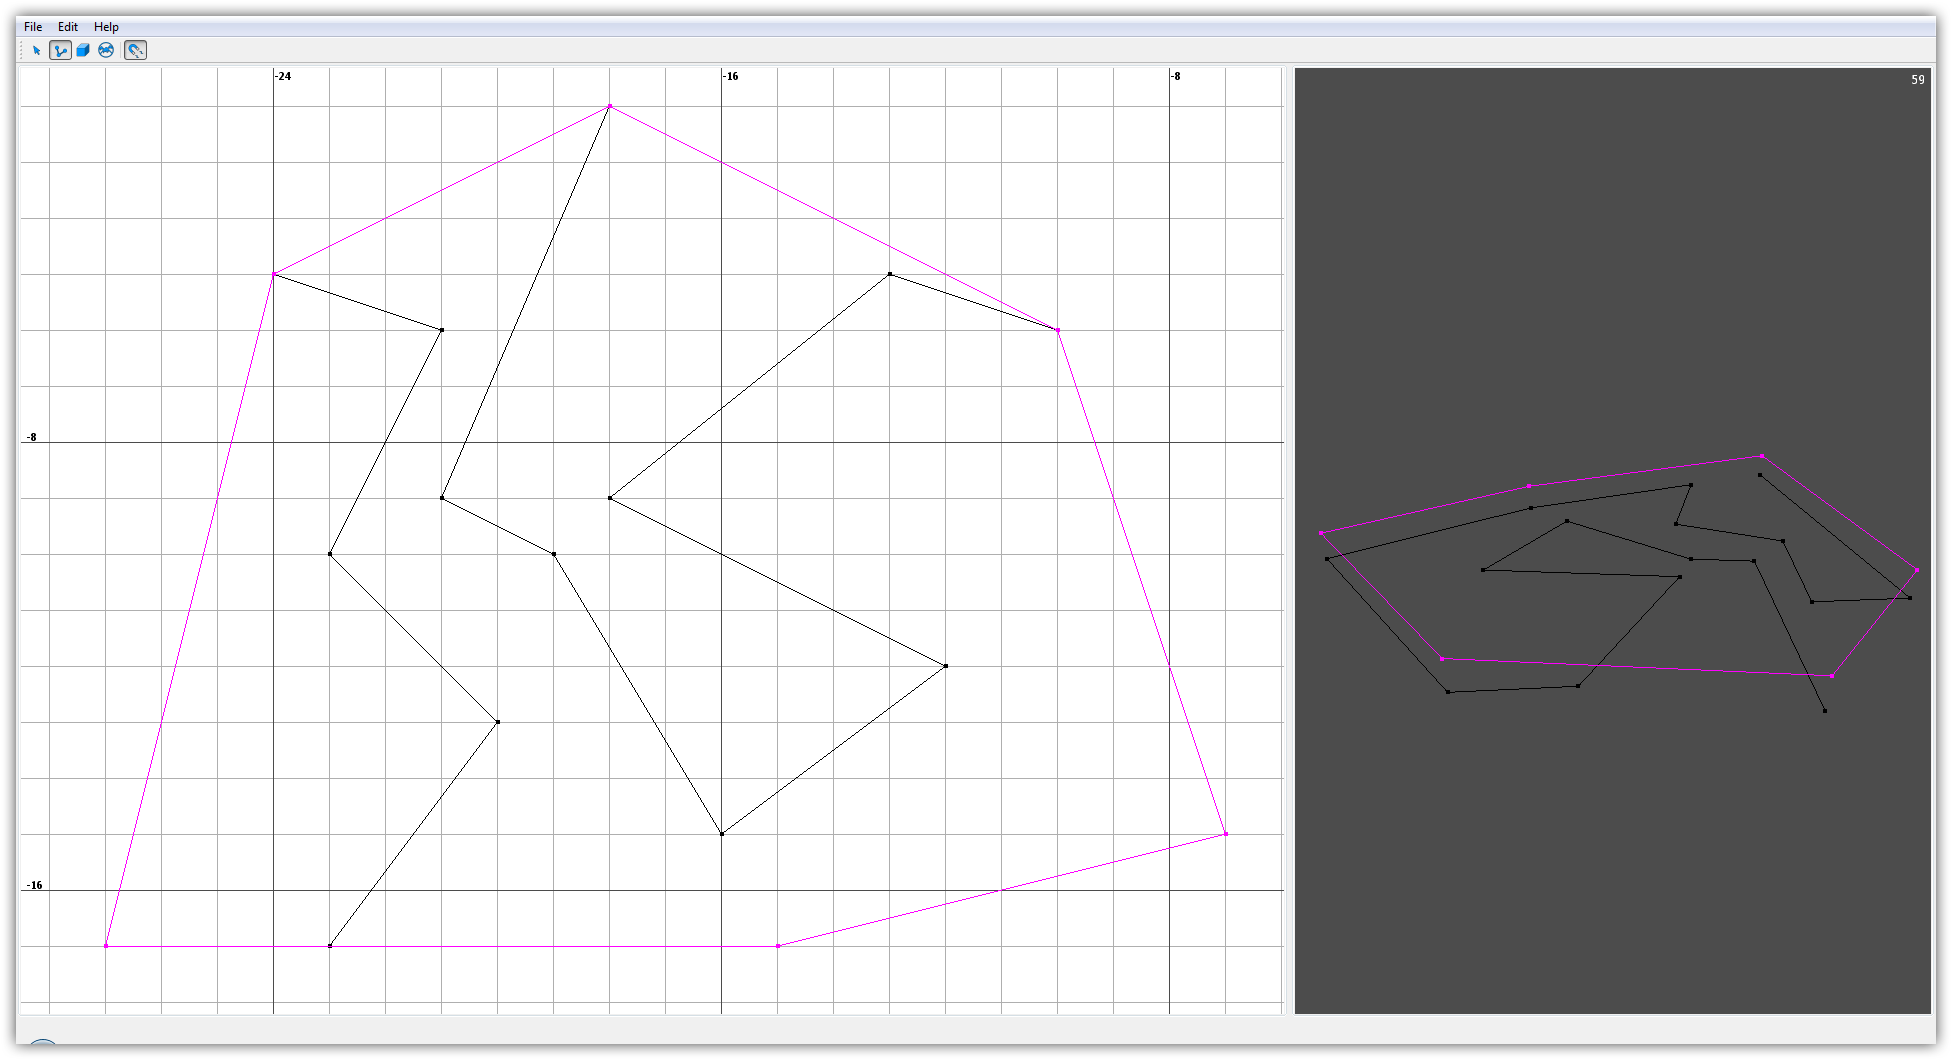
\includegraphics[width=\textwidth]{figures/melkman-output-1}
% 	\caption{Output polygon drawn on top of input polyline.} 
% 	\label{fig:melkman-output}
% \end{figure}  
% 
% The orthographic view provides a simple CAD interface, and the input buttons
% control which objects are created when the user clicks inside the view. One
% button allows the user to create polylines. The snapping toggle button
% determines whether the points created are integral. 
% 
% After clicking a few times to create a polyline, the user completes the object
% by right-clicking, and the polyline remains selected. Right-clicking again
% reveals a menu with various algorithms listed. With a few lines of code, we can 
% add Melkman to the list and specify that our new function should execute on
% the currently selected object when we click on it. 

%==============================================================================

% The DDAD workbench makes it easy for presenters and implementers to quickly
% visualize new geometric objects and algorithms. In this section, we overview
% using the workbench to implement a bare-bones visualization of Melkman's convex
% hull algorithm~\cite{melkman1987line}. First, we implement the basic data
% types used by the algorithm and augment their methods with visualization
% code. Second, we use these data types to implement Melkman's algorithm. 
% By visualizing the data types in an object-oriented way, we arrive at a
% clean implementation of the algorithm.

% The DDAD workbench can quickly visualize three-dimensional algorithms. In this
% section, we use the workbench to visualize an implementation of incremental
% delaunay triangulation. The presentation follows the same format as our previous
% case study. First, we review the basic data types used by the algorithm and
% show how to augment their methods with visualization code. Second, we use these
% data types to implement the algorithm.

%\subsection{Data Type Design and Implementation}



% This section reviews animating an incremental Delaunay triangulation algorithm.
% The algorithm is covered extensively in \cite{de2000computational}.  

%\subsection{Algorithm Overview}

% The algorithm uses the quadedge data structure~\cite{guibas1985primitives}.
% 
% \begin{mdframed}[linecolor=white, backgroundcolor=algback, frametitle={Algorithm
% Delaunay}] \begin{algorithmic}[1]
%     \Require A set $P$ of $n+1$ points in the plane.
%     \Ensure A Delaunay triangulation of $P$.
%     \vspace{0.75em}
%     \Procedure{Delaunay}{$P$}
%     \State Let $p_0$ be the lexicographically highest point of $P$.
%     \State Let $p_{-1}, p_{-2}$ be two points far away such that $P$ is
%     contained in the triangle $p_0p_{-1}p_{-2}$.
%     \State Initialize $\mathcal{T}$ as the triangulation consisting of the
%     single triangle $p_0p_{-1}p_{-2}$.
%     \State Compute a random permutation $p_1, p_2, \ldots, p_n$ of $P /
%     \{p_0\}$.
%     \For{$r = 1 \ldots n$}
%    \State derp
%     \EndFor \EndProcedure
% \end{algorithmic}
% \end{mdframed} 

% \subsection{Code Listing}
% 
% \lstinputlisting{code-samples/delaunay.cpp}
% 
% \subsection{Generating Input Data}
% 
% The user is given a button in the GUI and may browse to read in point sets
% stored in text files.


\FloatBarrier
\section{Lessons Learned and Future Directions} 
\label{sec:lessons-learned}

[todo]

% Implementing a geometric algorithm workbench is a challenging task with a rich
% set of problems encompassing a variety of disciplines. We converged on an
% interesting events design in which the user annotates observable objects to
% signal changes in their visual state. The user specifies visual state on points,
% line segments, and triangles, determines delay length between animation
% sequences, and directs the viewing camera while the animation runs.
% 	
% Many opportunities for improvement and further exploration exist. First,
% implementing existing plans of debugging controls affords an immediate
% improvement in the tool's usefulness. Second, allowing the presenter to specify
% sounds to accompany interesting events provides another means of conveying
% information. Finally, creating better abstractions of common data structures and
% investigating integration with existing debuggers reduces system invasiveness
% for the implementer.
 
\bibliographystyle{abbrv}
\bibliography{../../references}

\clearpage
\appendix
\FloatBarrier
\section{Appendix}

This section contains two types of information. First, there is
information about aspects of the workbench that should help users and
contributors understand its inner workings. Second, there is information that
can serve as background for some of the concepts found in the main paper. Much
of this section is mirrored on the DDAD wiki; areas for future work are captured
in issues on Github. References to issues are labeled with a triangle
($\triangle$) and the issue number.

%==============================================================================

\subsection{Adding New Geometric Types}\label{appdx:adding-new-geometric-types}

This section covers how to add new geometric types to the DDAD workbench.

\begin{enumerate} 
  \item Create a new header and implementation file under the geometry library
  folder. See folder structure (\ref{appdx:folder-structure}). File names are in
  lower case with underscores between words (e.g. \texttt{geometry/my\_geometric\_type.h}.)
  Smaller, closely related items should be placed in the same file to avoid
  proliferation of tiny fragment files (e.g. polyline and polygon types are both placed into
  files named \texttt{polygon.h/polygon.cpp.}) See the coding
  guidelines (\ref{appdx:coding-guidelines}) for more detail on naming
  conventions.
  \item Define the interface of your new geometric type. You may use the
  template provided in listing~\ref{geometric-type-template} or look to existing
  geometric types for guidance.
  Importantly, you must inherit from \texttt{Visual::Geometry}. Some things you
  should notice about the template:
  \begin{itemize}
    \item All files start with the license.% (\ref{appdx:license}). 
    \item Next is a short one-liner describing the file that uses the
    \href{http://www.stack.nl/~dimitri/doxygen/}{Doxygen} tag \texttt{@brief}.
    \item All header files use
    \href{http://en.wikipedia.org/wiki/Include\_guard}{include guards}. Include
    guards in the geometry project are prefixed with \texttt{GE\_} and workbench
    include guards are prefixed with \texttt{WB\_}. Next, add the name of your
    file in uppercase. All guards end with \texttt{\_H}.
    \item All files include \texttt{common.h} which includes system utilities
    and logging. Visual types include \texttt{visual.h} which defines the visual
    geometry interfaces.
    \item Geometric types are suffixed with their dimension and the underlying
    arithmetic type. For example, \texttt{\_2f} denotes a 2 dimensional object
    with single-precision floating-point coordinates. See the coding
    guidelines (\ref{appdx:coding-guidelines}) for a full suffix listing.
  \end{itemize}
%   \lstinputlisting[caption=Geometric Type Template,
%   label=geometric-type-template]{code-samples/geometric-type-template.cpp}
  \item Provide implementations of the default constructor, copy constructor,
  and destructor. The copy constructor is important to implement if you plan on
  returning a copy of your type from functions, e.g. \texttt{Melkman} returns a
  \texttt{Polygon\_2r}. If you have not implemented a copy constructor, you may
  experience double-destruction of returned visualization primitives.
  \item Implement your geometric type as you normally would.
  \item Augment the type's methods with visual signals to reflect the state of
  the object. For example, listing~\ref{polyline-push-back} shows that adding a
  point to a polyline also registers the point so it can be viewed.
%   \lstinputlisting[caption=Example of Augmented Method,
%   label=polyline-push-back]{code-samples/polyline-push-back.cpp}
  \item Define a scene object (\ref{appdx:scene-objects}) type in
  \texttt{workbench/scene.h} that corresponds to your geometric type. You may
  use the template in listing~\ref{scene-object-template}.
%   \lstinputlisting[caption=Scene Object Template,
%   label=scene-object-template]{code-samples/scene-object-template.cpp}
  \item Implement the \texttt{Select}, \texttt{Deselect}, and \texttt{Intersect}
  methods so that your object can be selected in the editor. Refer to
  picking (\ref{appdx:picking}) for more details.
  \item Add a button to the Create tab defining ways for the user to create your
  object. Add the button using Qt Designer by opening
  \texttt{workbench/forms/window\_main.ui}. The button should have a
  human-readable name for your object and an icon representation. Add your
  button to the \texttt{buttonGroup} with \texttt{Right-click -> Assign to
  button group}.
  \item  Create a custom \texttt{MyGeometricObjectCreationMethod} widget. Click
  on \texttt{File -> New File or Project}. You will see the dialog shown in
  figure~\ref{fig:creation-method}.
  \begin{figure}[H]
	\centering
	\shadowimage[width=\textwidth]{figures/gui-creation-method-new-file}
	\caption{Dialog for creating a new creation method widget.} 
	\label{fig:creation-method}
  \end{figure}
  \item Implement the \texttt{toggle} event handler for the button. Right-click
  on the button in Qt Designer and choose \texttt{Go to slot...} then
  \texttt{toggled(bool)}. This will automatically add the appropriate member
  functions onto the main window class and navigate you to the implementation
  stub in \texttt{qt\_window\_main.cpp}. Listing~\ref{creation-toggle-handler}
  shows the toggled handler for \texttt{Polyline\_2r} objects. Some things to notice:
%   \lstinputlisting[caption=Creation Button Toggle Handler,
%   label=creation-toggle-handler]{code-samples/creation-toggle-handler.cpp}
  \begin{itemize}
    \item All creation buttons must call \texttt{uncheckInputModeButtons()}
    since creation and input mode buttons are mutually exclusive.
    \item Use a static function variable for the \texttt{creation\_method}
    QWidget. The first time the button is \texttt{toggled(true)}, we create the
    widget and we destroy the widget when we are \texttt{toggled(false)}.
    \emph{Be sure to delete the widget to avoid a memory leak.}
    \item We set the input mode so that click events in the Orthographic Widget
    will be handled appropriately.
  \end{itemize}
\end{enumerate}

\lstinputlisting[float, caption=Geometric Type Template,
  label=geometric-type-template]{code-samples/geometric-type-template.cpp}

\lstinputlisting[float, caption=Example of Augmented Method,
  label=polyline-push-back]{code-samples/polyline-push-back.cpp}
  
\lstinputlisting[float, caption=Scene Object Template,
  label=scene-object-template]{code-samples/scene-object-template.cpp}
  
\lstinputlisting[float, caption=Creation Button Toggle Handler,
  label=creation-toggle-handler]{code-samples/creation-toggle-handler.cpp}
%==============================================================================

\FloatBarrier
\subsection{Coding Guidelines}\label{appdx:coding-guidelines}

Many organizations and individuals have taken the time to author style
guidelines for the C++ language. A thorough style document is an undertaking in
its own right; they may span many pages and include detailed rules, exceptions,
and justifications for both. For this project, it made sense to leverage the
work of others by adopting and customizing an existing set of guidelines:
\href{http://google-styleguide.googlecode.com/svn/trunk/cppguide.html}{Google's
C++ style guide}. \emph{Contributors should pay attention to coding style so
that we can keep the code uniform, clean, and easy to read.} 

\paragraph{Highlights.}

\begin{itemize}
  \item Strictly adhere to 80-char line widths.
  \item Use lowercase, underscore separated variable names instead of
  camelCase.
  \item Private member variables should be suffixed with an underscore:
  \texttt{my\_member\_var\_}.
\end{itemize}

\paragraph{Additions or Exceptions.}

\begin{itemize}
  \item Geometric types are suffixed with their dimension and underlying
  arithmetic type.
  \begin{itemize}
    \item \texttt{f} = single-precision floating-point
    \item \texttt{d} = double-precision floating-point
    \item \texttt{i} = MPIR integer
    \item \texttt{r} = MPIR rational
  \end{itemize}
\end{itemize}

%==============================================================================

\FloatBarrier
\subsection{Compiling}\label{appdx:compiling}

\begin{enumerate}
  \item Clone the repository. \texttt{git clone
  https://github.com/unc-compgeom/ddad.git}
  \item Install prerequisite software.
  \begin{itemize}
    \item
    \href{http://www.visualstudio.com/en-us/products/free-developer-offers-vs}{Visual Studio Community 2013}
    \item \href{http://www.cmake.org/download/}{CMake 2.8.12 or later}
    \item \href{http://www.qt.io/download-open-source/}{Qt 5.3 32-bit (Desktop
    OpenGL)}
  \end{itemize}
  \item Compile MPIR in \texttt{dependencies/mpir}.
  \item Open DDAD in QtCreator.
\end{enumerate}

%==============================================================================

\FloatBarrier
\subsection{Deploying}\label{appdx:deploying}

Deploying refers to the process of bundling together the workbench executable
with its dependencies for download by non-developers. Windows users should
perform 4 steps to use the DDAD Workbench.

\begin{enumerate}
  \item Install the MSVC redistributable package.
  \item Download a zip file from the website.
  \item Extract the zip file.
  \item Double-click the executable.
\end{enumerate}

This guide makes no assumptions about what is already installed. We could use an
installer to remove the burden of installing the MSVC package, but keeping
deployments to a simple zip file minimizes the barrier for new developers.

\paragraph{Test Setup.} In order to properly test whether your deployment will
work as expected, it is advisable to simulate the target user's machine and
attempt to follow the installation directions listed below. In particular, since
we assume a blank-slate installation, using VMWare to create a clean install of
Windows 7 x64 Home Premium is an easy way to verify the build and instructions.

Outside of advanced user analysis, assuming a blank slate install is about the
best we can do. In practice, users will have a variety of other software
installed that may cause conflicts with the software required to run the
workbench. These sorts of problems should be logged and documented.

\paragraph{Create the zip.} These instructions use absolute paths; please
substitute your own as appropriate.

\begin{itemize}
  \item Create an empty folder that will house your executable and associated
  DLL files.
  \item Copy the release .exe into the folder. You do not need the manifest
  file.
  \item Go into \texttt{C:/Qt/Qt5.1.1/5.1.1/msvc2010\_opengl/bin}
  \item Copy any required DLLs and paste them next to the .exe in your new
  folder. (If you encounter problems, copy all of them to ensure this step is
  not a source of problems. Once you get everything working, you can prune out
  unnecessary DLLs using Dependency Walker. For the default test application, I
  needed: Qt5Core.dll, Qt5Gui.dll, Qt5Widgets.dll, and all dll's prefixed with
  ``icu.'')
  \item Go into \texttt{C:/Qt/Qt5.1.1/5.1.1/msvc2010\_opengl/plugins/platforms}
  \item Copy qwindows.dll and paste it in \texttt{<your new folder>/platforms}.
  You have to perform this step for all applications, even if you don�t know
  what plugins are or don�t think your application is using any.
  \item Compress your new folder.
\end{itemize}

\paragraph{Find the right redistributable.} Qt packages an appropriate
redistributable installer with itself. Instead of hunting around for it on the
internet, we can provide users with Qt's to install.

\begin{enumerate}
  \item Go into \texttt{C:/Qt/Qt5.1.1/vcredist}
  \item You should see something like \texttt{vcredist\_sp1\_x86.exe}.
  \item Provide this file for users to install, as a separate download.
\end{enumerate}

\paragraph{Final process for end users.} After uploading the zipped installation
folder and the corresponding redistributable provided by Qt, the installation
process on the VMWare Windows 7 x64 machine looks like the following.

\begin{enumerate}
  \item Download \texttt{vcredist\_sp1\_x86.exe}.
  \item Run the installer, using all default settings.
  \item Download the zipped installation folder.
  \item Unzip.
  \item Double-click executable.
\end{enumerate}

\paragraph{Notes.} Getting this to work took me longer than expected due to two
problems. First, I had multiple Qt installations on my development machine,
which must have resulted in me copying the wrong dll�s or using the wrong
version of Qt Creator, or something. Uninstalling all versions of Qt, deleting
the corresponding folders, then installing only the version I wanted to use made
debugging much easier. Second, I had difficulty finding the right version of the
MSVC redistributable package on the web. Using the one provided by Qt helped
tremendously; it worked the first time.

%==============================================================================

\FloatBarrier
\subsection{Managing Dependencies}\label{appdx:dependencies}

The DDAD library and workbench share two dependencies:
\href{http://mpir.org/}{MPIR} and
\href{https://github.com/easylogging/easyloggingpp}{EasyLogging++}. MPIR is a
wrapper around GMP and provides arbitrary precision integer, rational, and
floating-point types. EasyLogging++ is a header-only logging library for C++.

\paragraph{The problem.} Many languages have well-supported dependency
management systems: Bower for JavaScript, npm for node.js, Maven and Gradle for
Java. There is currently no standardized way to do dependency management in C++.
This is due to a variety of reasons, including language implementation
differences (mixed support for language features), platform differences (some
platforms do not support exceptions), and compilation differences (static or
shared? debug or production?).
% \begin{quote}
% 	\begin{itemize}
% 	  \item Implementation differences - C++ is a complicated language, and
% 	  different implementations have historically varied in how well they support
% 	  it (how well they can correctly handle various moderate to advanced C++
% 	  code). So there's no guarantee that a library could be built in a particular
% 	  implementation.
% 	  \item Platform differences - Some platforms may not support exceptions. There
% 	  are different implementations of the standard library, with various pros and
% 	  cons. Unlike Java's standardized library, Windows and POSIX APIs can be quite
% 	  different. The filesystem isn't even a part of Standard C++.
% 	  \item Compilation differences - Static or shared? Debug or production build?
% 	  Enable optional dependencies or not? Unlike Java, which has very stable
% 	  bytecode, C++'s lack of a standard ABI means that code may not link properly,
% 	  even if built for the same platform by the same compiler.
% % 	  \item Build system differences - Makefiles? (If so, GNU Make, or something
% % 	  else?) Autotools? CMake? Visual Studio project files? Something else?
% % 	  \item Historical concerns - Because of C's and C++'s age, popular libraries
% % 	  like zlib predate build systems like Maven by quite a bit. Why should zlib
% % 	  switch to some hypothetical C++ build system when what it's doing works? How
% % 	  can a newer, higher-level library switch to some hypothetical build system if
% % 	  it depends on libraries like zlib?
% 	\end{itemize}
% \end{quote}

\paragraph{Possible solutions.} Below, we discuss possible solutions to managing
dependencies and give pros and cons of each approach.

\begin{enumerate}
  \item Since MPIR and EasyLogging++ both have officially maintained GitHub
  repositories, we could use \texttt{git subtree} to bring the source code into
  our repository. Git will maintain a direct link to each repository, and
  updating each dependency can be accomplished with \texttt{git subtree pull}.
  Atlassian has an in-depth article on how to use \texttt{git subtree}
  \href{http://blogs.atlassian.com/2013/05/alternatives-to-git-submodule-git-subtree/}{here}.
  
  Pros: Makes updating dependencies easy. Does not require special
  initialization after user clones DDAD repository. Cross-platform: user is
  responsible for compiling on their machine.
  
  Cons: Requires user to compile dependencies before compiling DDAD. Increased
  learning curve: developers must be adept at git in case things go awry.
  
%   \begin{table}[h]
%     \begin{tabularx}{\textwidth}{XX}
% 	\toprule
% 	Pros & Cons \\
% 	\midrule
% 	\begin{itemize}
% 	  \item Makes updating dependencies easy
% 	  \item Does not require special initialization after user clones DDAD
% 	  repository
% 	  \item Cross-platform: user is responsible for compiling on their machine 
% 	\end{itemize} &
% 	\begin{itemize}
% 	  \item Requires user to compile dependencies before compiling DDAD
% 	  \item Increased learning curve: developers must be adept at git in case
% 	  things go awry
% 	\end{itemize} \\
%     \bottomrule    
% 	\end{tabularx}
%   \end{table}  

  \item Manually take a snapshot of each dependency and copy the source into our
  repository. This does not involve unusual git commands and there will be no
  link to the original dependency repository.
  
  Pros: Low learning curve: anyone can copy over files. Does not require special
  initialization after user clones DDAD repository. Cross-platform: user is
  responsible for compiling on their machine.
  
  Cons: Requires user to compile dependencies before compiling DDAD. Updating
  dependencies is a manual process. Documenting dependency versions is a manual
  process.

%   \begin{table}[h]
%     \begin{tabularx}{\textwidth}{XX}
% 	\toprule
% 	Pros & Cons \\
% 	\midrule
% 	\begin{itemize}
% 	  \item Low learning curve: anyone can copy over files
% 	  \item Does not require special initialization after user clones DDAD
% 	  repository
% 	  \item Cross-platform: user is responsible for compiling on their machine 
% 	\end{itemize} &
% 	\begin{itemize}
% 	  \item Requires user to compile dependencies before compiling DDAD
% 	  \item Updating dependencies is a manual process
% 	  \item Documenting dependency versions is a manual process
% 	\end{itemize} \\
%     \bottomrule    
% 	\end{tabularx}
%   \end{table} 
 
  \item Manually build a snapshot of each dependency and copy the binaries into
  our repository. This does not involve unusual git commands and there will be
  no link to the original dependency repository. If the user is on supported
  OS's and compiler versions then they do not need to compile dependencies
  themselves. 
  
  Pros: Low learning curve, anyone can copy over files. Does not
  require special initialization after user clones DDAD. Users on supported
  platforms do not need to compile dependencies before compiling DDAD. 
  
  Cons: Not cross-platform: binaries are tied to specific operating systems and
  specific compiler versions. Updating dependencies is laborious: developers
  must compile a new snapshot for all OS and compiler version combinations we
  wish to support. Documenting dependency versions is a manual process.
  
% 	  compiling DDAD
% 	  repository
%   \begin{table}[h]
%     \begin{tabularx}{\textwidth}{XX}
% 	\toprule
% 	Pros & Cons \\
% 	\midrule
% 	\begin{itemize}
% 	  \item Low learning curve: anyone can copy over files
% 	  \item Does not require special initialization after user clones DDAD
% 	  repository
% 	  \item Users on supported platforms do not need to compile dependencies before
% 	  compiling DDAD 
% 	\end{itemize} &
% 	\begin{itemize}
% 	  \item Not cross-platform: binaries are tied to specific operating systems and
% 	  specific compiler versions
% 	  \item Updating dependencies is laborious: developers must compile a new
% 	  snapshot for all OS and compiler version combinations we wish to support
% 	  \item Documenting dependency versions is a manual process
% 	\end{itemize} \\
%     \bottomrule    
% 	\end{tabularx}
%   \end{table}

\end{enumerate}

\paragraph{Our solution.} We chose 2. This way we strike a balance between
remaining cross-platform withou  creating too high of a barrier to entry for new
developers. This is justified as follows:

\begin{itemize}
  \item We wish to keep the number of dependencies low. Thus, we do not expect
  to be adding many more beyond MPIR and EasyLogging++.
  \item MPIR is a stable project that has existed for many years. Although there
  is active development and GitHub repository, there are not major feature
  changes that would significantly change the functionality as far as DDAD is
  concerned.
  \item EasyLogging++ is a single-header library, so updating this dependency is
  just a matter of downloading one file and copying it into the project.
\end{itemize}

%==============================================================================

\FloatBarrier
\subsection{Folder Structure}\label{appdx:folder-structure}

Files are laid out according to the following hierarchy.

\begin{itemize}
  \item \texttt{/geometry} - geometry library, includes linear algebra,
  arithmetic, geometric primitives, intersection tests, data structures and
  algorithms.
  \item \texttt{/workbench} - workbench system built using Qt. Contains two
  subfolders:
  \begin{itemize}
    \item \texttt{/resources} - graphics such as application icon and splash
    screen
    \item \texttt{/forms} - Qt ui files for use with Qt Designer. These allow
    the programmer to visually design various screens in the application.
  \end{itemize}
  \item \texttt{/utility} - contains useful code that may be used in any other
  project. e.g. logging.
  \item \texttt{/documentation} - \LaTeX~source files for various types of
  documentation.
  \item \texttt{/dependencies} - 3rd party libraries, e.g. MPIR.
\end{itemize}

%==============================================================================

\FloatBarrier
\subsection{GUI Overview}\label{appdx:gui-overview}

The Graphical User Interface (GUI) comprises 7 components: the menubar, the
toolbar, the orthographic widget, the perspective widget, the interactive panel,
the statusbar, and the console.

% ![GUI Overview](http://cs.unc.edu/~freeman/DDAD/media/gui-overview.png)
\paragraph{Menubar.} The menubar comprises 3 high-level menus: File, Edit, and
Help. It exists primarily as a scaffold for future functionality.

\begin{itemize}
	\item File. The File menu is currently empty but
	\href{https://github.com/unc-compgeom/DDAD/issues/6}{issue $\triangle$ 6}
	specifies saving and loading of files. To do this, we need a mechanism for
	serializing and deserializing the scene, which is a major undertaking.
    \item Edit. The Edit menu contains one element, Preferences (there are
    issues to add duplicating and copy/paste.) Clicking Preferences will open a
    dialog which is split into 3 major panels. On the left is a list of
    subsections. The list currently contains only Grid Settings. On the right is
    a detailed view of the selected subsection. This detail view is
    parameterized by the list on the left. Finally, the bottom contains 4
    buttons: Default, Cancel, Apply, and Ok. The most interesting of these is
    Default, which requires the application to somehow define defaults. Settings
    \& Defaults bring up the notion of a configuration file (e.g. .ini). While
    currently there are not many settings, the dialog sets forth a framework
    into which developers can add new configurations settings.
    \item Help. The Help menu contains two simple elements. The first is a link
    to the user manual (the wiki). The second is an About dialog that provides
    information about the program version and a link to the project webpage.
\end{itemize}

\paragraph{Toolbar.} The toolbar comprises 4 elements: 3 buttons to control
input mode (Select, Translate, and Rotate), and 1 button to toggle snapping to
grid. The three input mode buttons are mutually exclusive with one another and
with the creation buttons in the interactive panel. The select mode is initially
activated and allows the user to pick one object at a time via left-clicking in
the orthographic and perspective views.
\href{https://github.com/unc-compgeom/DDAD/issues/8}{Issue $\triangle$ 8}
specifies multiple-object selection,
\href{https://github.com/unc-compgeom/DDAD/issues/9}{issue $\triangle$ 9}
specifies the rotation mode, and
\href{https://github.com/unc-compgeom/DDAD/issues/10}{issue $\triangle$ 10}
specifies the translation mode.

\paragraph{Orthographic widget.} The orthographic widget allows users to
precisely create and manipulate objects against the backdrop of an integer grid.
The integer grid has minor and major grid lines. Minor lines are drawn in a
lighter color. Major lines occur after a certain number of minor lines - the
default is 8.

Users are able to zoom in and out and pan around the grid. As the user zooms
out, the grid adapts so that the lines are not drawn too close together. At the
highest zoom level, minor lines are drawn 1 unit apart. After the user zooms out
a ways, the grid adapts to draw minor lines 8 units apart. After more zooming,
the grid adapts to draw minor lines 64 units apart, and so on.

\paragraph{Perspective widget.} The perspective widget allows the user to
control a 3D perspective camera that renders the current scene. Users may change
the camera's orientation and move forward (W), backward (S), left (A), right (D)
up (E), and down (C).

\paragraph{Interactive panel.} The interactive panel comprises three tabs:
Create, Modify, and Compute.

The create tab is open by default. It initially has only a gallery of geometric
objects. The buttons in the gallery are mutually exclusive with one another and
with the input mode buttons in the toolbar. Once the user selects one of the
geometric objects, an additional ``Creation Method'' panel will appear with
additional options. The options are parameterized by the selected object type;
often these methods will overlap (e.g. clicking inside the orthographic view to
create a point set or polyline), but may be unique (e.g. a polytope may have a
user-defined length, width, and height). Each method will be listed in a
dropdown menu at the top of the panel. As the user changes between methods,
method-specific controls will appear below the dropdown. For example, when
``Click'' is selected, explanatory text appears; if you change the selection to
``File,'' then the explanatory text will be replaced with a file chooser and
``Generate'' button.

The modify tab is meant to let the user choose the \emph{selection granularity},
or the level at which operations are applied. For example, a polytope is
composed of vertices, edges, and faces. Each of these, along with the whole
polytope, are selectable levels of granularity. When ``edges'' is selected,
picking operations will choose from only the object's edges, when ``vertices''
is selected, picking operations will choose from only the object's vertices, and
so on. Most of this functionality is not yet implemented, but is specified in
\href{https://github.com/unc-compgeom/DDAD/issues/7}{issue $\triangle$ 7}.

The compute tab is composed of the name of the selected object and a drop down
menu of applicable algorithms. The dropdown of algorithms follows the same logic
as the creation method dropdown, meaning that as you change your selection
relevant parameters will appear below. Once the user is with the algorithm
selection and any parameters, they would like to execute the algorithm. For
this, we provide a set of media controls. In particular, they may click the
``Run'' button which will begin algorithm execution. Once the algorithm is
running, editing controls will be disabled.

\paragraph{Statusbar.} The statusbar provides a way of sending messages to the
user, depending on application context. For example, when the user is creating a
polyline, the application cycles through 2 different states. First, the user
needs to click in the orthographic view to position the initial vertex, so we
might simply display: ``Left-click in the orthographic view to place first
vertex.'' Second, the user can either place additional vertices in the same
fashion, or terminate the polyline by right-clicking; the status bar should be
updated to reflect the user's options: ``Left-click again to add more vertices,
or right-click to terminate polyline.'' Finally, after the user right-clicks to
terminate, we transition back to creating a new polyline, so the message should
update as well.

The main window defines a slot for updating the statusbar message (\texttt{void
onUpdateStatusBarMsg(const QString\& status)}). To trigger the handler from
another QObject, you must ensure that the instance is connected to the main
window, then emit an appropriate signal. For more information, see Qt's
documentation on
\href{http://qt-project.org/doc/qt-4.8/signalsandslots.html}{signals and slots} and
\href{http://qt-project.org/doc/qt-4.8/qstatusbar.html}{QStatusBar}.

\paragraph{Console.}

The console is designed to provide non-developers with useful information in
case they experience unexpected (but non-terminal) behavior. By logging to the
console, developers can ask these users to inspect the console to understand the
application behavior. The console is not meant as a replacement of the IDE
console. By default, the console is hidden from view, but may be expanded at any
time.

%==============================================================================

\FloatBarrier
\subsection{Predicates}\label{appdx:predicates}
 
Given three points in the plane, $p$, $q$, and $r$, the 2D orientation predicate
$\textsc{Orient2D}(p, q, r)$ answers the question, ``is $r$ to the left, right,
or on the oriented line $pq$?'' We may write it as the sign of a 2-by-2
determinant, where negative is left, positive is right, and zero is on. In
particular, we have 
\[
\textsc{Orient2D}(p, q, r) = \textsc{Sign}
\left(
	\begin{vmatrix} 
		x_p-x_r & y_p-y_r \\ 
		x_q-x_r & y_q-y_r 
	\end{vmatrix} 
\right).
\]
 

Given 4 points in the plane, $p, q, r$, and $s$, the predicate
$\textsc{InCircle}(p, q, r, s)$ answers the question, ``is $s$ inside, outside,
or on the oriented circle through $p, q$, and $r$?'' We may write it as the sign
of a 4-by-4 determinant, where negative is inside, positive is outside, and zero
is on. In particular, we have

\[ 
\textsc{InCircle}(p, q, r, s) = \textsc{Sign}\left(
\begin{vmatrix}
	x_p & y_p & x_p^2 + y_p^2 & 1 \\
    x_q & y_q & x_q^2 + y_q^2 & 1\\
    x_r & y_r & x_r^2 + y_r^2 & 1\\
    x_s & y_s & x_s^2 + y_s^2 & 1\\
\end{vmatrix}
\right).
\]

%==============================================================================
\clearpage
\FloatBarrier
\subsection{Scene Objects}\label{appdx:scene-objects}

The scene is composed of a collection of \emph{scene objects}, all of which must
implement the \texttt{ISceneObject} interface. This interface obligates scene
objects to have a name, color, be able to intersect itself with a 3D ray for
picking (\ref{appdx:picking}), and define what it means to be selected or
deselected.

\lstinputlisting[caption=ISceneObject Interface,
  label=isceneobject-interface]{code-samples/isceneobject.cpp}
 
%==============================================================================

\FloatBarrier
\subsection{Intersection Types}\label{appdx:intersection-types}

The geometry library defines a number of intersection types that represent the
intersection between two objects. It makes sense to create full types for
intersections because there is often quite a bit of information to capture (is
the intersection empty, a point, a line segment, a ray? when did the
intersection occur?). Perhaps more interestingly, intersection types nicely
align the C++ concept of constructors with our geometric concept of a
construction. The design is inspired by David Eberly's
\href{http://www.geometrictools.com/Source/Intersection2D.html}{geometric tools}.

Intersection types are placed in the \texttt{Intersection} namespace and follow
a naming convention: simply repeat the names of the two types being intersected.
The \texttt{Line\_2rLine\_2r} type is a good example:

\lstinputlisting[float, caption=Line\_2rLine\_2r Intersection Type,
  label=intersection-line2rline2r]{code-samples/intersection-line2rline2r.cpp}

%==============================================================================

\FloatBarrier
\subsection{Picking}\label{appdx:picking}

\paragraph{The Problem.} Picking is the process of selecting the foremost object
in a view that lies under a user's mouse click. In our case, we are given an 
input mouse click from either the orthographic or perspective views, and must
choose from among the scene objects.

\paragraph{Possible Solutions.}

\begin{enumerate}
  \item Color each object a unique color, render a frame, and use the
  final pixel color to determine which object to select. OpenGL provides a
  picking mode that does this.
  \item Generate a 3D world-space ray from the mouse click and intersect this
  ray with scene objects to determine which object it intersects first. 
\end{enumerate}

\paragraph{Our Solution.} We chose method 2 because it was more straightforward
to get working than 1 and probably more efficient. In particular, we take click
events from the orthographic and perspective views and convert them into a 3D
worldspace ray. We iterate over all scene objects (there is no hierarchical
acceleration structure) and produce \texttt{Ray\_3rSceneObject} intersection
objects. These objects are quite simple, see listing
\ref{intersection-ray3rsceneobject}. We hill climb over the intersection times
to determine which object intersected first.

\lstinputlisting[caption=Ray\_3rSceneObject Intersection Type,
  label=intersection-ray3rsceneobject]{code-samples/intersection-ray3rsceneobject.cpp}

\paragraph{Selecting and Deselecting.} The \texttt{Select} method should usually
just highlight the object's edges and vertices with the global selection color
(for the moment, methods all just use \texttt{Visual::Color::SKYBLUE},
\href{https://github.com/unc-compgeom/DDAD/issues/3}{issue $\triangle$ 3}
specifies a solution.) Listing \ref{intersection-select} shows an example
\texttt{Select} implementation from \texttt{ScenePolyline\_2r}.

\lstinputlisting[float, caption=Example Select Method,
  label=intersection-select]{code-samples/intersection-select.cpp}

%==============================================================================

\FloatBarrier
\subsection{Order-independent Transparency}\label{appdx:oit}

\paragraph{The problem.} Rendering transparent surfaces is not as easy as one
might imagine. Most ways of compositing layers of translucent pixels on top of
one another show \emph{order-dependency}, meaning that the order that surfaces
are rendered can affect the final pixel color. This problem arises because the
terms in the blending equation are not commutative, so different orders of
compositing result in different pixel colors.

\paragraph{Possible solutions.} There are a number of techniques to achieve
\emph{order-independent transparency} (OIT), including
A-buffers~\cite{carpenter1984buffer}, depth
peeling~\cite{everitt2001interactive}, dual depth
peeling~\cite{bavoil2008order}, and others. Hardware manufacturers are moving
toward providing special hardware to solve OIT quickly for real-time rendering
applications. OIT techniques may be categorized into exact and approximate
methods. The ground truth is the industry-accepted OVER operator. Examples of
approximate techniques include McGuire's weighted, blended
OIT~\cite{mcguire2013weighted}.

\paragraph{Our solution.}
 
The workbench does not currently have a full implementation of OIT available,
but the functionality is specified in
\href{https://github.com/unc-compgeom/DDAD/issues/4}{issue $\triangle$ 4}.
However, the main framework is in place. Most OIT techniques require a
separation between opaque and transparent geometry. The visual interface
supports transparent materials, and when we generate vertex buffers to send to
OpenGL for rendering, opaque and transparent vertices are segregated into
different buffers. This means that it is easy to render opaque objects before
transparent ones.


\end{document}

\endinput












































% The workbench is composed of two major systems: the geometry kernel and the
% visualizer. The geometry kernel houses arithmetic (MPIR bignums, number
% theoretic functions), linear algebra (vectors and matrices), low-level geometric
% primitives (points, line segments, and triangles), high-level geometric types
% (polylines, polygons, subdivisions, etc.), and geometric algorithms (convex
% hull, integer hull, delaunay triangulation, etc.).
%
%
% The geometry kernel encapsulates geometric algorithm implementations.
%
% The visualizer encapsulates the visual display of geometric algorithms.


% Geometric algorithms are typically designed and analyzed using the Real-RAM
% model of computation \cite{preparata1977convex}. In other words, these
% algorithms assume that the numerical data in geometric objects are exact
% values in $\mathbb{R}$ that can be stored and retrieved in constant time, and
% that arithmetic involving these values is performed in constant time. From a
% practical point of view, it may seem like an odd or frustrating decision to
% assume access to infinite precision real arithmetic, given that digital
% computers are finite objects. From a theoretical point of view, this is a
% sensible choice given that for subsets of $\mathbb{R}$, such as the rational
% numbers $\mathbb{Q}$, many fundamental geometric axioms no longer hold.


% \subsection{Report Overview}
%
% Lacking a suitable workbench, we decided to build our own. This report details
% the resulting system and is composed of two major sections. First, we state
% workbench desiderata, explain current workbench capabilities, and show how these
% capabilities support the desiderata. Second, we overview our workbench
% architecture. We discuss at a high level how the two major components -- the
% geometry kernel and the visualizer -- work together to animate geometric
% algorithms. Finally, we conclude by reviewing lessons learned from the project
% and identify avenues for future work.

% \subsubsection{Forrest geometric computing environments}
%
% Forrest suggested the geometry community start building ``geometric computing
% environments'' in the late 1980's~\cite{forrest1987computational,
% forrest1988geometric}.

% \subsubsection{LINETool (1988)}
%
% Yap and Ericson discuss the design of LINETool, a geometric editor. They
% differentiate their tool from automated theorem provers for geometry. Designed
% in support of exact computation.~\cite{ericson1988design}

% There is a long history of geometric workbench systems. In the late 1980's
% Forrest identified the need for ``geometric computing environments'' that would
% provide both a library of geometric algorithms and a supporting user interface
% for animation and debugging~\cite{forrest1987computational,
% forrest1988geometric}.
%
%
%
%
% Concurrently, Yap and Ericson designed LINEtool, a
% ``geometric editor" that allowed users to exactly specify and render geometric
% constructions~\cite{ericson1988design}. Soon after, three projects were underway
% that sought to provide a geometric computing environment: XYZ
% GeoBench~\cite{schorn1991robust}, Workbench~\cite{epstein1994workbench}, and the
% Library of Efficient Data Types and Algorithms (LEDA)~\cite{mehlhorn1989leda}.
% XYZ GeoBench and Workbench most fully fit the definition of a geometric
% computing environment, while LEDA focused primarily on the development of a
% library.
%
% Dobkin and Hausner~\cite{hausner1999animation} review four geometric
% visualization systems: Workbench \cite{epstein1994workbench}, XYZ
% GeoBench \cite{schorn1991implementing, schorn1991robust}, Geomview
% \cite{amenta1995geomview}, and GASP \cite{tal1995visualization}.

% Schorn joined
% Nievergelt's group at UNC Chapel Hill in 1986 and completed his MSc in
% Computer Science in 1988. Schorn and Nievergelt returned to ETH Zurich in
% 1989, with Schorn eventually completing his PhD in 1991.
% written in Object Pascal

% \subsection{General algorithm animation}
%
% \paragraph{BALSA} \cite{brown1984system}
%
% \paragraph{BALSA-II}
%
% \paragraph{Zeus}
%
% \paragraph{AnimA}
%
% \paragraph{TANGO} \cite{stasko1990tango}
%
% \paragraph{POLKA} \cite{stasko1995polka}
%
% \paragraph{SAMBA} \cite{stasko1995samba}
